\documentclass[runningheads]{llncs}


\usepackage{graphicx}

\usepackage{array}
\usepackage{multirow}
%\usepackage{amssymb}
\usepackage{xspace}
\usepackage{color,soul}
\usepackage{adjustbox}
\usepackage{comment}
\usepackage{url}
\usepackage[utf8]{inputenc}
\usepackage{algorithm}
\usepackage{algorithmic}
\usepackage{float}
\usepackage{enumitem}
\usepackage{amsmath}

\newcommand{\method}{SHIELD\xspace}
\renewcommand{\algorithmicrequire}{\textbf{Input:}}
\renewcommand{\algorithmicensure}{\textbf{Output:}}
\newcommand{\new}[1]{\textcolor{red}{#1}}
\usepackage{color}

%% \BibTeX command to typeset BibTeX logo in the docs
%\AtBeginDocument{%
%  \providecommand\BibTeX{{%
%    Bib\TeX}}}

%% Rights management information.  This information is sent to you
%% when you complete the rights form.  These commands have SAMPLE
%% values in them; it is your responsibility as an author to replace
%% the commands and values with those provided to you when you
%% complete the rights form.
%
\begin{document}
\title{\method: APT Detection and Intelligent Explanation Using LLM}
%
\titlerunning{\method: APT Detection and Intelligent Explanation Using LLM}
% If the paper title is too long for the running head, you can set
% an abbreviated paper title here
%
\author{Parth Atulbhai Gandhi \and Prasanna N. Wudali \and Yonatan Amaru \and 
Yuval Elovici \and
Asaf Shabtai}
%
\authorrunning{Gandhi et al.}
% First names are abbreviated in the running head.
% If there are more than two authors, 'et al.' is used.
%
\institute{Ben-Gurion University of the Negev}
%
\maketitle


\begin{abstract}
Advanced persistent threats (APTs) are sophisticated cyber attacks that can remain undetected for extended periods, making their mitigation particularly challenging. 
Given their persistence, significant effort is required to detect them and respond effectively. 
Existing provenance-based attack detection methods often lack interpretability and suffer from high false positive rates, while investigation approaches are either supervised or limited to known attacks. 
To address these challenges, we introduce \method, a novel approach that combines statistical anomaly detection and graph-based analysis with the contextual analysis capabilities of large language models (LLMs). 
\method leverages the implicit knowledge of LLMs to uncover hidden attack patterns in provenance data, while reducing false positives and providing clear, interpretable attack descriptions. 
This reduces analysts' alert fatigue and makes it easier for them to understand the threat landscape. 
Our extensive evaluation demonstrates \method's effectiveness and computational efficiency in real-world scenarios. 
\method was shown to outperform state-of-the-art methods, achieving higher precision and recall. 
\method's integration of anomaly detection, LLM-driven contextual analysis, and advanced graph-based correlation establishes a new benchmark for APT detection.

\keywords{Attack detection, Large language model, provenance graph}

\end{abstract}


\section{Introduction}
\label{sec:introduction}
The business processes of organizations are experiencing ever-increasing complexity due to the large amount of data, high number of users, and high-tech devices involved \cite{martin2021pmopportunitieschallenges, beerepoot2023biggestbpmproblems}. This complexity may cause business processes to deviate from normal control flow due to unforeseen and disruptive anomalies \cite{adams2023proceddsriftdetection}. These control-flow anomalies manifest as unknown, skipped, and wrongly-ordered activities in the traces of event logs monitored from the execution of business processes \cite{ko2023adsystematicreview}. For the sake of clarity, let us consider an illustrative example of such anomalies. Figure \ref{FP_ANOMALIES} shows a so-called event log footprint, which captures the control flow relations of four activities of a hypothetical event log. In particular, this footprint captures the control-flow relations between activities \texttt{a}, \texttt{b}, \texttt{c} and \texttt{d}. These are the causal ($\rightarrow$) relation, concurrent ($\parallel$) relation, and other ($\#$) relations such as exclusivity or non-local dependency \cite{aalst2022pmhandbook}. In addition, on the right are six traces, of which five exhibit skipped, wrongly-ordered and unknown control-flow anomalies. For example, $\langle$\texttt{a b d}$\rangle$ has a skipped activity, which is \texttt{c}. Because of this skipped activity, the control-flow relation \texttt{b}$\,\#\,$\texttt{d} is violated, since \texttt{d} directly follows \texttt{b} in the anomalous trace.
\begin{figure}[!t]
\centering
\includegraphics[width=0.9\columnwidth]{images/FP_ANOMALIES.png}
\caption{An example event log footprint with six traces, of which five exhibit control-flow anomalies.}
\label{FP_ANOMALIES}
\end{figure}

\subsection{Control-flow anomaly detection}
Control-flow anomaly detection techniques aim to characterize the normal control flow from event logs and verify whether these deviations occur in new event logs \cite{ko2023adsystematicreview}. To develop control-flow anomaly detection techniques, \revision{process mining} has seen widespread adoption owing to process discovery and \revision{conformance checking}. On the one hand, process discovery is a set of algorithms that encode control-flow relations as a set of model elements and constraints according to a given modeling formalism \cite{aalst2022pmhandbook}; hereafter, we refer to the Petri net, a widespread modeling formalism. On the other hand, \revision{conformance checking} is an explainable set of algorithms that allows linking any deviations with the reference Petri net and providing the fitness measure, namely a measure of how much the Petri net fits the new event log \cite{aalst2022pmhandbook}. Many control-flow anomaly detection techniques based on \revision{conformance checking} (hereafter, \revision{conformance checking}-based techniques) use the fitness measure to determine whether an event log is anomalous \cite{bezerra2009pmad, bezerra2013adlogspais, myers2018icsadpm, pecchia2020applicationfailuresanalysispm}. 

The scientific literature also includes many \revision{conformance checking}-independent techniques for control-flow anomaly detection that combine specific types of trace encodings with machine/deep learning \cite{ko2023adsystematicreview, tavares2023pmtraceencoding}. Whereas these techniques are very effective, their explainability is challenging due to both the type of trace encoding employed and the machine/deep learning model used \cite{rawal2022trustworthyaiadvances,li2023explainablead}. Hence, in the following, we focus on the shortcomings of \revision{conformance checking}-based techniques to investigate whether it is possible to support the development of competitive control-flow anomaly detection techniques while maintaining the explainable nature of \revision{conformance checking}.
\begin{figure}[!t]
\centering
\includegraphics[width=\columnwidth]{images/HIGH_LEVEL_VIEW.png}
\caption{A high-level view of the proposed framework for combining \revision{process mining}-based feature extraction with dimensionality reduction for control-flow anomaly detection.}
\label{HIGH_LEVEL_VIEW}
\end{figure}

\subsection{Shortcomings of \revision{conformance checking}-based techniques}
Unfortunately, the detection effectiveness of \revision{conformance checking}-based techniques is affected by noisy data and low-quality Petri nets, which may be due to human errors in the modeling process or representational bias of process discovery algorithms \cite{bezerra2013adlogspais, pecchia2020applicationfailuresanalysispm, aalst2016pm}. Specifically, on the one hand, noisy data may introduce infrequent and deceptive control-flow relations that may result in inconsistent fitness measures, whereas, on the other hand, checking event logs against a low-quality Petri net could lead to an unreliable distribution of fitness measures. Nonetheless, such Petri nets can still be used as references to obtain insightful information for \revision{process mining}-based feature extraction, supporting the development of competitive and explainable \revision{conformance checking}-based techniques for control-flow anomaly detection despite the problems above. For example, a few works outline that token-based \revision{conformance checking} can be used for \revision{process mining}-based feature extraction to build tabular data and develop effective \revision{conformance checking}-based techniques for control-flow anomaly detection \cite{singh2022lapmsh, debenedictis2023dtadiiot}. However, to the best of our knowledge, the scientific literature lacks a structured proposal for \revision{process mining}-based feature extraction using the state-of-the-art \revision{conformance checking} variant, namely alignment-based \revision{conformance checking}.

\subsection{Contributions}
We propose a novel \revision{process mining}-based feature extraction approach with alignment-based \revision{conformance checking}. This variant aligns the deviating control flow with a reference Petri net; the resulting alignment can be inspected to extract additional statistics such as the number of times a given activity caused mismatches \cite{aalst2022pmhandbook}. We integrate this approach into a flexible and explainable framework for developing techniques for control-flow anomaly detection. The framework combines \revision{process mining}-based feature extraction and dimensionality reduction to handle high-dimensional feature sets, achieve detection effectiveness, and support explainability. Notably, in addition to our proposed \revision{process mining}-based feature extraction approach, the framework allows employing other approaches, enabling a fair comparison of multiple \revision{conformance checking}-based and \revision{conformance checking}-independent techniques for control-flow anomaly detection. Figure \ref{HIGH_LEVEL_VIEW} shows a high-level view of the framework. Business processes are monitored, and event logs obtained from the database of information systems. Subsequently, \revision{process mining}-based feature extraction is applied to these event logs and tabular data input to dimensionality reduction to identify control-flow anomalies. We apply several \revision{conformance checking}-based and \revision{conformance checking}-independent framework techniques to publicly available datasets, simulated data of a case study from railways, and real-world data of a case study from healthcare. We show that the framework techniques implementing our approach outperform the baseline \revision{conformance checking}-based techniques while maintaining the explainable nature of \revision{conformance checking}.

In summary, the contributions of this paper are as follows.
\begin{itemize}
    \item{
        A novel \revision{process mining}-based feature extraction approach to support the development of competitive and explainable \revision{conformance checking}-based techniques for control-flow anomaly detection.
    }
    \item{
        A flexible and explainable framework for developing techniques for control-flow anomaly detection using \revision{process mining}-based feature extraction and dimensionality reduction.
    }
    \item{
        Application to synthetic and real-world datasets of several \revision{conformance checking}-based and \revision{conformance checking}-independent framework techniques, evaluating their detection effectiveness and explainability.
    }
\end{itemize}

The rest of the paper is organized as follows.
\begin{itemize}
    \item Section \ref{sec:related_work} reviews the existing techniques for control-flow anomaly detection, categorizing them into \revision{conformance checking}-based and \revision{conformance checking}-independent techniques.
    \item Section \ref{sec:abccfe} provides the preliminaries of \revision{process mining} to establish the notation used throughout the paper, and delves into the details of the proposed \revision{process mining}-based feature extraction approach with alignment-based \revision{conformance checking}.
    \item Section \ref{sec:framework} describes the framework for developing \revision{conformance checking}-based and \revision{conformance checking}-independent techniques for control-flow anomaly detection that combine \revision{process mining}-based feature extraction and dimensionality reduction.
    \item Section \ref{sec:evaluation} presents the experiments conducted with multiple framework and baseline techniques using data from publicly available datasets and case studies.
    \item Section \ref{sec:conclusions} draws the conclusions and presents future work.
\end{itemize}
\section{Related Works}
\label{sec:related_works}


\noindent\textbf{Diffusion-based Video Generation. }
The advancement of diffusion models \cite{rombach2022high, ramesh2022hierarchical, zheng2022entropy} has led to significant progress in video generation. Due to the scarcity of high-quality video-text datasets \cite{Blattmann2023, Blattmann2023a}, researchers have adapted existing text-to-image (T2I) models to facilitate text-to-video (T2V) generation. Notable examples include AnimateDiff \cite{Guo2023}, Align your Latents \cite{Blattmann2023a}, PYoCo \cite{ge2023preserve}, and Emu Video \cite{girdhar2023emu}. Further advancements, such as LVDM \cite{he2022latent}, VideoCrafter \cite{chen2023videocrafter1, chen2024videocrafter2}, ModelScope \cite{wang2023modelscope}, LAVIE \cite{wang2023lavie}, and VideoFactory \cite{wang2024videofactory}, have refined these approaches by fine-tuning both spatial and temporal blocks, leveraging T2I models for initialization to improve video quality.
Recently, Sora \cite{brooks2024video} and CogVideoX \cite{yang2024cogvideox} enhance video generation by introducing Transformer-based diffusion backbones \cite{Peebles2023, Ma2024, Yu2024} and utilizing 3D-VAE, unlocking the potential for realistic world simulators. Additionally, SVD \cite{Blattmann2023}, SEINE \cite{chen2023seine}, PixelDance \cite{zeng2024make} and PIA \cite{zhang2024pia} have made significant strides in image-to-video generation, achieving notable improvements in quality and flexibility.
Further, I2VGen-XL \cite{zhang2023i2vgen}, DynamicCrafter \cite{Xing2023}, and Moonshot \cite{zhang2024moonshot} incorporate additional cross-attention layers to strengthen conditional signals during generation.



\noindent\textbf{Controllable Generation.}
Controllable generation has become a central focus in both image \citep{Zhang2023,jiang2024survey, Mou2024, Zheng2023, peng2024controlnext, ye2023ip, wu2024spherediffusion, song2024moma, wu2024ifadapter} and video \citep{gong2024atomovideo, zhang2024moonshot, guo2025sparsectrl, jiang2024videobooth} generation, enabling users to direct the output through various types of control. A wide range of controllable inputs has been explored, including text descriptions, pose \citep{ma2024follow,wang2023disco,hu2024animate,xu2024magicanimate}, audio \citep{tang2023anytoany,tian2024emo,he2024co}, identity representations \citep{chefer2024still,wang2024customvideo,wu2024customcrafter}, trajectory \citep{yin2023dragnuwa,chen2024motion,li2024generative,wu2024motionbooth, namekata2024sg}.


\noindent\textbf{Text-based Camera Control.}
Text-based camera control methods use natural language descriptions to guide camera motion in video generation. AnimateDiff \cite{Guo2023} and SVD \cite{Blattmann2023} fine-tune LoRAs \cite{hu2021lora} for specific camera movements based on text input. 
Image conductor\cite{li2024image} proposed to separate different camera and object motions through camera LoRA weight and object LoRA weight to achieve more precise motion control.
In contrast, MotionMaster \cite{hu2024motionmaster} and Peekaboo \cite{jain2024peekaboo} offer training-free approaches for generating coarse-grained camera motions, though with limited precision. VideoComposer \cite{wang2024videocomposer} adjusts pixel-level motion vectors to provide finer control, but challenges remain in achieving precise camera control.

\noindent\textbf{Trajectory-based Camera Control.}
MotionCtrl \cite{Wang2024Motionctrl}, CameraCtrl \cite{He2024Cameractrl}, and Direct-a-Video \cite{yang2024direct} use camera pose as input to enhance control, while CVD \cite{kuang2024collaborative} extends CameraCtrl for multi-view generation, though still limited by motion complexity. To improve geometric consistency, Pose-guided diffusion \cite{tseng2023consistent}, CamCo \cite{Xu2024}, and CamI2V \cite{zheng2024cami2v} apply epipolar constraints for consistent viewpoints. VD3D \cite{bahmani2024vd3d} introduces a ControlNet\cite{Zhang2023}-like conditioning mechanism with spatiotemporal camera embeddings, enabling more precise control.
CamTrol \cite{hou2024training} offers a training-free approach that renders static point clouds into multi-view frames for video generation. Cavia \cite{xu2024cavia} introduces view-integrated attention mechanisms to improve viewpoint and temporal consistency, while I2VControl-Camera \cite{feng2024i2vcontrol} refines camera movement by employing point trajectories in the camera coordinate system. Despite these advancements, challenges in maintaining camera control and scene-scale consistency remain, which our method seeks to address. It is noted that 4Dim~\cite{watson2024controlling} introduces absolute scale but in  4D novel view synthesis (NVS) of scenes.



\chapter{Implementation}{\label{ch:implementation}}
In this chapter, we present the implementation of the final product. We start by discussing how the four steps introduced in \hyperref[ch:high_level_approach]{chapter \ref*{ch:high_level_approach}} are integrated. We then outline the main system components of our score follower, presenting each as an independent, self-contained module. We then combine this into an overall system architecture and finally introduce the open-source score renderer used to display the score and evaluate the score follower.       

% \section{Aims and Requirements}
% The overall aim of the score follower was to 


\section{Score Follower Framework Details}
Our score follower conforms to the high-level framework presented in \hyperref[section:score_follower_framework]{section \ref*{section:score_follower_framework}}. In step 1, two score features are extracted from a MIDI file (see \hyperref[subsection:midi]{subsection \ref*{subsection:midi}}), namely MIDI note numbers\footnote{\href{https://inspiredacoustics.com/en/MIDI_note_numbers_and_center_frequencies}{https://inspiredacoustics.com/en/MIDI\_note\_numbers\_and\_center\_frequencies}} (corresponding to pitch) and note onsets (corresponding to duration). In step 2, the audio is streamed (whether from a file or into a microphone) and audioframes that exceed some predefined energy threshold are extracted. Here, audioframes are groups of contiguous audio samples, whose length can be specified by the argument \verb|frame_length|, usually between 800 and 2000 samples. The period between consecutive audioframes can also be defined by the argument \verb|hop_length|, typically between 2000 and 5000 audio samples. In step 3, score following is performed via a `Windowed' Viterbi algorithm (see  \hyperref[subsection:adjusting_viterbi]{subsection \ref*{subsection:adjusting_viterbi}}) which uses the Gaussian Process (GP) log marginal likelihoods (LMLs) for emission probabilities (see \hyperref[section:state_duration_model]{section \ref*{section:state_duration_model}}) and a state duration model for transition probabilities (see \hyperref[section:state_duration_model]{section \ref*{section:state_duration_model}}). Finally, in step 4 we render our results using an adapted version of the open source user interface, \textit{Flippy Qualitative Testbench}.

\section{Following Modes}
Two modes are available to the user: Pre-recorded Mode and Live Mode. The former requires a pre-recorded $\verb|.wav|$ file, whereas the latter takes an input stream of audio via the device's microphone. Note that both modes are still forms of score following, as opposed to score alignment, since in each mode we receive audioframes at the sampling rate, not all at once.\\

Live Mode offers a practical example of a score follower, displaying a score and position marker which a musician can read off while playing. However, this mode is not suitable for evaluation because the input and results cannot be easily replicated. Even ignoring repeatability, Live Mode is not suitable for one-off testing since a musician using this application may be influenced by the movement of the marker. For instance, the performer may speed up if the score follower `gets ahead' or slow down if the position marker lags or `gets lost'. To avoid this, we use Pre-recorded Mode when evaluating the performance of our score follower. Furthermore, Pre-recorded Mode offers the advantage of testing away from the music room, providing the opportunity to evaluate a variety of recordings available online. 

\section{System Architecture}
Our guiding principle for development was to build modular code in order to create a streamlined system where each component performs a specific task independently. This structure facilitates easy testing and debugging. \hyperref[fig:black_box]{Figure \ref*{fig:black_box}} presents a high-level architecture diagram, where each black box abstracts a key component of the score follower. When operating in Pre-recorded Mode, there is the option to stream the recording during run-time, which outputs to the device's speakers (as indicated by the dashed lines).

\begin{figure}[H]
    \centering
    \includegraphics[width=1\textwidth]{figs/Part_4_Implementation_And_Results/black_box.png}
    \caption{Abstracted system architecture diagram displaying inputs in grey, the 4 main components of the score follower in black and the outputs in green.}
    \label{fig:black_box}
\end{figure}

\subsection{Score Preprocessor}
The architecture for the Score Preprocesor is given in \hyperref[fig:score_preprocessor]{Figure \ref*{fig:score_preprocessor}}. First, MIDI note number and note onset times are extracted from each MIDI event. Simultaneous notes can be gathered into states and returned as a time-sorted list of lists called \verb|score|, where each element of the outer list is a list of simultaneous note onsets. Similarly, a list of note durations calculated as the time difference between consecutive states is returned as \verb|times_to_next|. Finally, all covariance matrices are precalculated and stored in a dictionary, where the key of the dictionary is determined by the notes present. This is because the distribution of notes and chords in a score is not random: notes tend to belong to a home \gls{key} and melodies tend to be repeated or related (similar to subject fields in speech processing). Therefore, states tend to be reused often, allowing us to achieve amortised time and space savings (by avoiding repeated calculation of the same covariance matrices). 

\begin{figure}[H]
    \centering
    \includegraphics[width=1\textwidth]{figs/Part_3_Implementation/Stage_2_Alignment/score_preprocessor.png}
    \caption{System architecture diagram representing the Score Preprocessor with inputs in grey, processes in blue and objects in yellow.}
    \label{fig:score_preprocessor}
\end{figure}


\subsection{Audio Preprocessor}
The architecture for the Audio Preprocessor is illustrated in \hyperref[fig:audio_preprocessor]{Figure \ref*{fig:audio_preprocessor}}. In Pre-recorded Mode, the Slicer receives a $\verb|.wav|$ file and returns audioframes separated by the \verb|hop_length|. These audioframes are periodically added to a multiprocessing queue, \verb|AudioFramesQueue|, to simulate real-time score following. In Live Mode, we use the python module \verb|sounddevice| to receive a stream of audio, using a periodic callback function to place audioframes on \verb|AudioFramesQueue|. 

\begin{figure}[H]
    \centering
    \includegraphics[width=1\textwidth]{figs/Part_4_Implementation_And_Results/audio_preprocessor.png}
    \caption{System architecture diagram representing the Audio Preprocessor with inputs in grey, processes in blue and objects in yellow.}
    \label{fig:audio_preprocessor}
\end{figure}

\subsection{Follower and Backend}
The joint Follower and Backend architecture diagram is shown in \hyperref[fig:follwer_and_backend]{Figure \ref*{fig:follwer_and_backend}}. The Viterbi Follower (detailed in \hyperref[subsection:adjusting_viterbi]{section \ref*{subsection:adjusting_viterbi}}) calculates the most probable state in the score, given audioframes continually taken from \verb|AudioFramesQueue|. These states are placed on another multiprocessing queue, the \verb|FollowerOutputQueue|, for the Backend to process and send. This prevents any bottle-necking occurring at the Follower stage. The Backend first sets up a UDP connection and then reads off values from \verb|FollowerOutputQueue|, sending them via UDP packets to the score renderer.

\begin{figure}[H]
    \centering
    \includegraphics[width=1\textwidth]{figs/Part_4_Implementation_And_Results/follower_and_backend.png}
    \caption{System architecture diagram representing the Follower and Backend processes with processes in blue, objects in yellow and outputs in green.}
    \label{fig:follwer_and_backend}
\end{figure}

\subsection{Player}
In Pre-recorded Mode, the Player sets up a new process and begins streaming the recording once the Follower process begins. This provides a baseline for testing purposes, as a trained musician can observe the score position marker and judge how well it matches the music. 

\subsection{Overall System Architecture}
The overall system architecture is presented in \hyperref[fig:overall_system_architecture]{Figure \ref*{fig:overall_system_architecture}}. Since the Follower runs a real-time, time sensitive process, parallelism is employed to reduce the total system latency. We use two \verb|multiprocessing| queues\footnote{\href{https://docs.python.org/3/library/multiprocessing.html}{https://docs.python.org/3/library/multiprocessing.html}} to avoid bottle-necking, which allows us to run 4 concurrent processes (Audio Preprocessor, Follower, Backend, and Audio Player). Hence, this architecture allows the components to run independently of one another to avoid blocking. Furthermore, this allows the system to take advantage of the multiple cores and high computational power offered by most modern machines.  

\begin{figure}[H]
    \centering
    \includegraphics[width=1\textwidth]{figs/Part_4_Implementation_And_Results/overall_score_follower_2.png}
    \caption{System architecture diagram representing the overall score follower running in Pre-recorded mode, with inputs in grey, processes in blue, objects in yellow and outputs in green.}
    \label{fig:overall_system_architecture}
\end{figure}


\section{Rendering Results}{\label{section:renderer}}
To visualise the results of our score follower, we adapted an open source tool for testing different score followers.\footnote{\href{https://github.com/flippy-fyp/flippy-qualitative-testbench/blob/main/README.md}{https://github.com/flippy-fyp/flippy-qualitative-testbench/blob/main/README.md}} \hyperref[fig:flippy_example]{Figure \ref*{fig:flippy_example}} shows the user interface of the score position renderer, where the green bar indicates score position. 

\begin{figure}[H]
    \centering
    \includegraphics{figs/Part_4_Implementation_And_Results/example_renderer.png}
    \caption{Screenshot of the score renderer user interface which displays a score (here we show a keyboard arrangement of \textit{O Haupt voll Blut und Wunden} by Bach). The green marker represents the score follower position.}
    \label{fig:flippy_example}
\end{figure}



\definecolor{darkgreen}{rgb}{0.0, 0.5, 0.0}
\definecolor{violet}{rgb}{0.56, 0.0, 1.0}
\section{Evaluation}
We apply our methodology to derive counterfactual policies for various MDPs, addressing three main research questions: (1) how does our policy's performance compare to the Gumbel-max SCM approach; (2) how do the counterfactual stability and monotonicity assumptions impact the probability bounds; and (3) how fast is our approach compared with the Gumbel-max SCM method?

\begin{figure*}
    \centering
    %
    \resizebox{0.6\textwidth}{!}{
        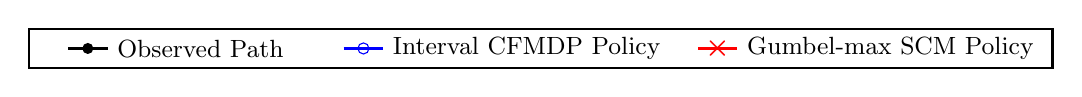
\begin{tikzpicture}[scale=1.0, every node/.style={scale=1.0}]
            \draw[thick, black] (-3, -0.25) rectangle (10, 0.25);
            %
            \draw[black, line width=1pt] (-2.5, 0.0) -- (-2,0.0);
            \fill[black] (-2.25,0.0) circle (2pt); %
            \node[right] at (-2,0.0) {\small Observed Path};
            
            %
            \draw[blue, line width=1pt] (1.0,0.0) -- (1.5,0.0);
            \node[draw=blue, circle, minimum size=4pt, inner sep=0pt] at (1.25,0.0) {}; %
            \node[right] at (1.5,0.0) {\small Interval CFMDP Policy};
            
            %
            \draw[red, line width=1pt] (5.5,0) -- (6,0);
            \node[red] at (5.75,0) {$\boldsymbol{\times}$}; %
            \node[right] at (6,0) {\small Gumbel-max SCM Policy};
        \end{tikzpicture}
    }\\
    %
    \subfigure[\footnotesize Lowest cumulative reward: Interval CFMDP ($312$), Gumbel-max SCM ($312$)]{%
        \resizebox{0.76\columnwidth}{!}{
             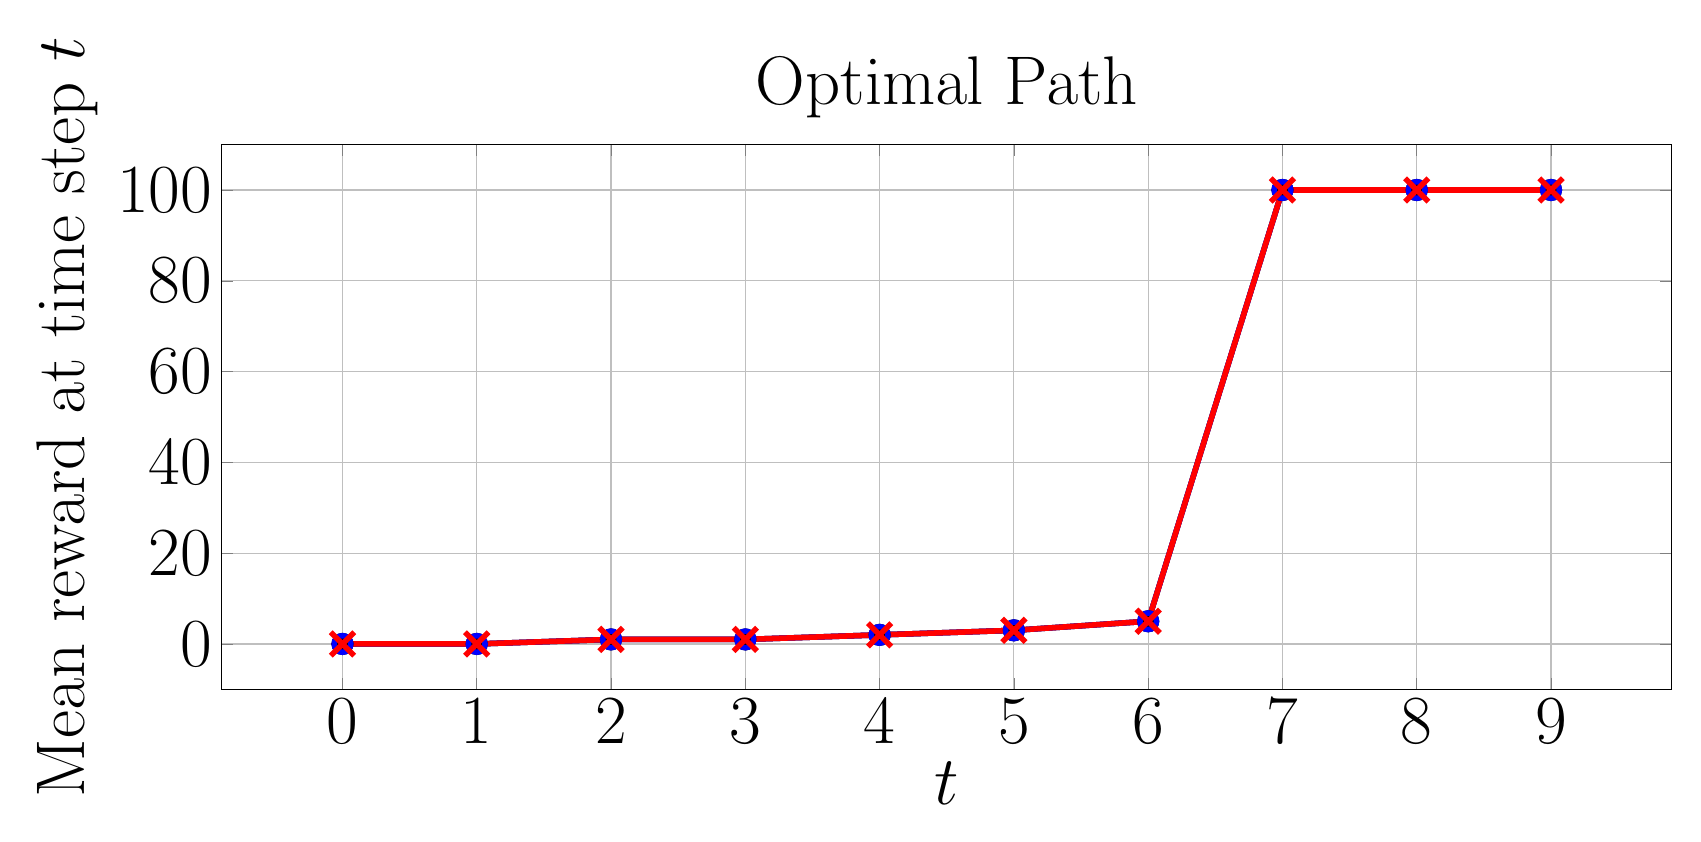
\begin{tikzpicture}
                \begin{axis}[
                    xlabel={$t$},
                    ylabel={Mean reward at time step $t$},
                    title={Optimal Path},
                    grid=both,
                    width=20cm, height=8.5cm,
                    every axis/.style={font=\Huge},
                    %
                ]
                \addplot[
                    color=black, %
                    mark=*, %
                    line width=2pt,
                    mark size=3pt,
                    error bars/.cd,
                    y dir=both, %
                    y explicit, %
                    error bar style={line width=1pt,solid},
                    error mark options={line width=1pt,mark size=4pt,rotate=90}
                ]
                coordinates {
                    (0, 0.0)  +- (0, 0.0)
                    (1, 0.0)  +- (0, 0.0) 
                    (2, 1.0)  +- (0, 0.0) 
                    (3, 1.0)  +- (0, 0.0)
                    (4, 2.0)  +- (0, 0.0)
                    (5, 3.0) +- (0, 0.0)
                    (6, 5.0) +- (0, 0.0)
                    (7, 100.0) +- (0, 0.0)
                    (8, 100.0) +- (0, 0.0)
                    (9, 100.0) +- (0, 0.0)
                };
                %
                \addplot[
                    color=blue, %
                    mark=o, %
                    line width=2pt,
                    mark size=3pt,
                    error bars/.cd,
                    y dir=both, %
                    y explicit, %
                    error bar style={line width=1pt,solid},
                    error mark options={line width=1pt,mark size=4pt,rotate=90}
                ]
                 coordinates {
                    (0, 0.0)  +- (0, 0.0)
                    (1, 0.0)  +- (0, 0.0) 
                    (2, 1.0)  +- (0, 0.0) 
                    (3, 1.0)  +- (0, 0.0)
                    (4, 2.0)  +- (0, 0.0)
                    (5, 3.0) +- (0, 0.0)
                    (6, 5.0) +- (0, 0.0)
                    (7, 100.0) +- (0, 0.0)
                    (8, 100.0) +- (0, 0.0)
                    (9, 100.0) +- (0, 0.0)
                };
                %
                \addplot[
                    color=red, %
                    mark=x, %
                    line width=2pt,
                    mark size=6pt,
                    error bars/.cd,
                    y dir=both, %
                    y explicit, %
                    error bar style={line width=1pt,solid},
                    error mark options={line width=1pt,mark size=4pt,rotate=90}
                ]
                coordinates {
                    (0, 0.0)  +- (0, 0.0)
                    (1, 0.0)  +- (0, 0.0) 
                    (2, 1.0)  +- (0, 0.0) 
                    (3, 1.0)  +- (0, 0.0)
                    (4, 2.0)  +- (0, 0.0)
                    (5, 3.0) +- (0, 0.0)
                    (6, 5.0) +- (0, 0.0)
                    (7, 100.0) +- (0, 0.0)
                    (8, 100.0) +- (0, 0.0)
                    (9, 100.0) +- (0, 0.0)
                };
                \end{axis}
            \end{tikzpicture}
         }
    }
    \hspace{1cm}
    \subfigure[\footnotesize Lowest cumulative reward: Interval CFMDP ($19$), Gumbel-max SCM ($-88$)]{%
         \resizebox{0.76\columnwidth}{!}{
            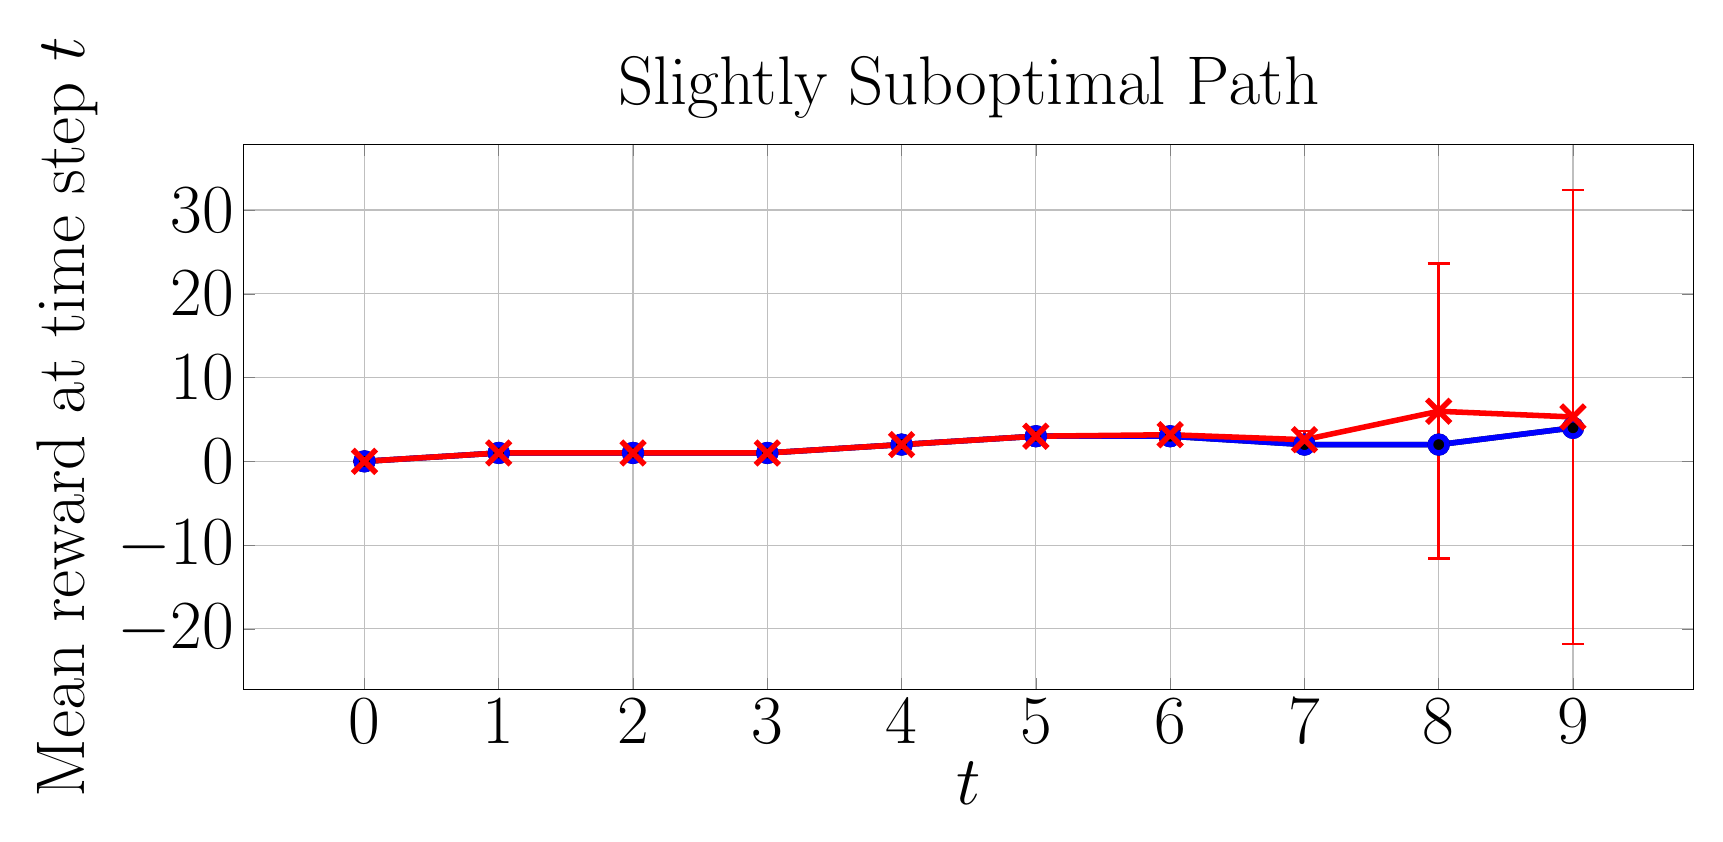
\begin{tikzpicture}
                \begin{axis}[
                    xlabel={$t$},
                    ylabel={Mean reward at time step $t$},
                    title={Slightly Suboptimal Path},
                    grid=both,
                    width=20cm, height=8.5cm,
                    every axis/.style={font=\Huge},
                    %
                ]
                \addplot[
                    color=black, %
                    mark=*, %
                    line width=2pt,
                    mark size=3pt,
                    error bars/.cd,
                    y dir=both, %
                    y explicit, %
                    error bar style={line width=1pt,solid},
                    error mark options={line width=1pt,mark size=4pt,rotate=90}
                ]
              coordinates {
                    (0, 0.0)  +- (0, 0.0)
                    (1, 1.0)  +- (0, 0.0) 
                    (2, 1.0)  +- (0, 0.0) 
                    (3, 1.0)  +- (0, 0.0)
                    (4, 2.0)  +- (0, 0.0)
                    (5, 3.0) +- (0, 0.0)
                    (6, 3.0) +- (0, 0.0)
                    (7, 2.0) +- (0, 0.0)
                    (8, 2.0) +- (0, 0.0)
                    (9, 4.0) +- (0, 0.0)
                };
                %
                \addplot[
                    color=blue, %
                    mark=o, %
                    line width=2pt,
                    mark size=3pt,
                    error bars/.cd,
                    y dir=both, %
                    y explicit, %
                    error bar style={line width=1pt,solid},
                    error mark options={line width=1pt,mark size=4pt,rotate=90}
                ]
              coordinates {
                    (0, 0.0)  +- (0, 0.0)
                    (1, 1.0)  +- (0, 0.0) 
                    (2, 1.0)  +- (0, 0.0) 
                    (3, 1.0)  +- (0, 0.0)
                    (4, 2.0)  +- (0, 0.0)
                    (5, 3.0) +- (0, 0.0)
                    (6, 3.0) +- (0, 0.0)
                    (7, 2.0) +- (0, 0.0)
                    (8, 2.0) +- (0, 0.0)
                    (9, 4.0) +- (0, 0.0)
                };
                %
                \addplot[
                    color=red, %
                    mark=x, %
                    line width=2pt,
                    mark size=6pt,
                    error bars/.cd,
                    y dir=both, %
                    y explicit, %
                    error bar style={line width=1pt,solid},
                    error mark options={line width=1pt,mark size=4pt,rotate=90}
                ]
                coordinates {
                    (0, 0.0)  +- (0, 0.0)
                    (1, 1.0)  +- (0, 0.0) 
                    (2, 1.0)  +- (0, 0.0) 
                    (3, 1.0)  +- (0, 0.0)
                    (4, 2.0)  += (0, 0.0)
                    (5, 3.0)  += (0, 0.0)
                    (6, 3.17847) += (0, 0.62606746) -= (0, 0.62606746)
                    (7, 2.5832885) += (0, 1.04598233) -= (0, 1.04598233)
                    (8, 5.978909) += (0, 17.60137623) -= (0, 17.60137623)
                    (9, 5.297059) += (0, 27.09227512) -= (0, 27.09227512)
                };
                \end{axis}
            \end{tikzpicture}
         }
    }\\[-1.5pt]
    \subfigure[\footnotesize Lowest cumulative reward: Interval CFMDP ($14$), Gumbel-max SCM ($-598$)]{%
         \resizebox{0.76\columnwidth}{!}{
             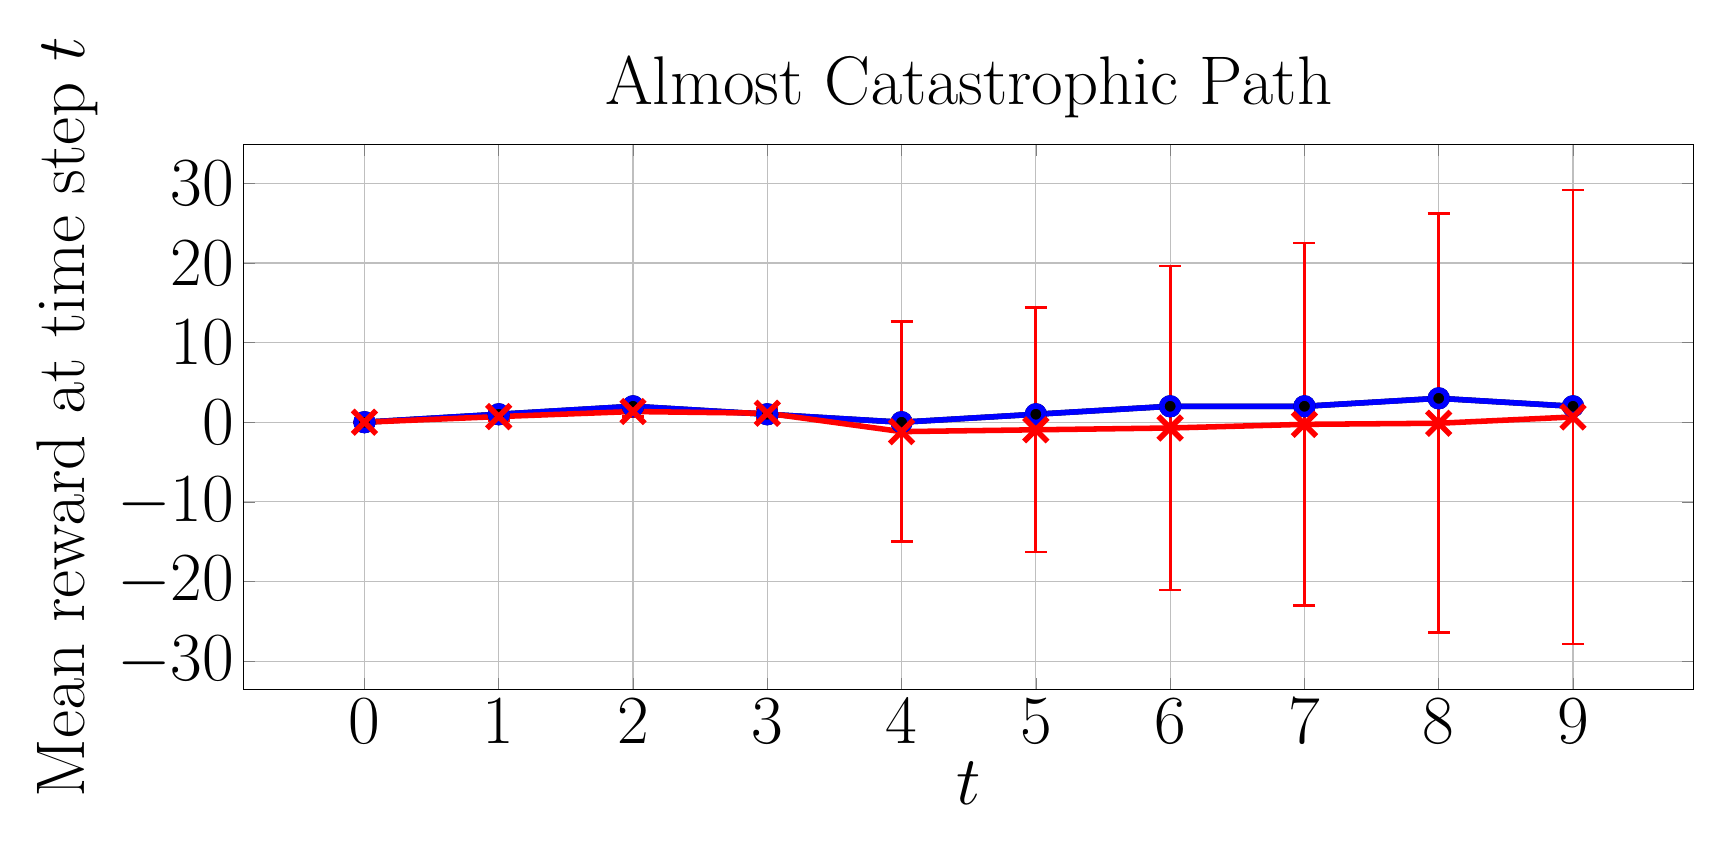
\begin{tikzpicture}
                \begin{axis}[
                    xlabel={$t$},
                    ylabel={Mean reward at time step $t$},
                    title={Almost Catastrophic Path},
                    grid=both,
                    width=20cm, height=8.5cm,
                    every axis/.style={font=\Huge},
                    %
                ]
                \addplot[
                    color=black, %
                    mark=*, %
                    line width=2pt,
                    mark size=3pt,
                    error bars/.cd,
                    y dir=both, %
                    y explicit, %
                    error bar style={line width=1pt,solid},
                    error mark options={line width=1pt,mark size=4pt,rotate=90}
                ]
                coordinates {
                    (0, 0.0)  +- (0, 0.0)
                    (1, 1.0)  +- (0, 0.0) 
                    (2, 2.0)  +- (0, 0.0) 
                    (3, 1.0)  +- (0, 0.0)
                    (4, 0.0)  +- (0, 0.0)
                    (5, 1.0) +- (0, 0.0)
                    (6, 2.0) +- (0, 0.0)
                    (7, 2.0) +- (0, 0.0)
                    (8, 3.0) +- (0, 0.0)
                    (9, 2.0) +- (0, 0.0)
                };
                %
                \addplot[
                    color=blue, %
                    mark=o, %
                    line width=2pt,
                    mark size=3pt,
                    error bars/.cd,
                    y dir=both, %
                    y explicit, %
                    error bar style={line width=1pt,solid},
                    error mark options={line width=1pt,mark size=4pt,rotate=90}
                ]
                coordinates {
                    (0, 0.0)  +- (0, 0.0)
                    (1, 1.0)  +- (0, 0.0) 
                    (2, 2.0)  +- (0, 0.0) 
                    (3, 1.0)  +- (0, 0.0)
                    (4, 0.0)  +- (0, 0.0)
                    (5, 1.0) +- (0, 0.0)
                    (6, 2.0) +- (0, 0.0)
                    (7, 2.0) +- (0, 0.0)
                    (8, 3.0) +- (0, 0.0)
                    (9, 2.0) +- (0, 0.0)
                };
                %
                \addplot[
                    color=red, %
                    mark=x, %
                    line width=2pt,
                    mark size=6pt,
                    error bars/.cd,
                    y dir=both, %
                    y explicit, %
                    error bar style={line width=1pt,solid},
                    error mark options={line width=1pt,mark size=4pt,rotate=90}
                ]
                coordinates {
                    (0, 0.0)  +- (0, 0.0)
                    (1, 0.7065655)  +- (0, 0.4553358) 
                    (2, 1.341673)  +- (0, 0.67091621) 
                    (3, 1.122926)  +- (0, 0.61281824)
                    (4, -1.1821935)  +- (0, 13.82444042)
                    (5, -0.952399)  +- (0, 15.35195457)
                    (6, -0.72672) +- (0, 20.33508414)
                    (7, -0.268983) +- (0, 22.77861454)
                    (8, -0.1310835) +- (0, 26.31013314)
                    (9, 0.65806) +- (0, 28.50670214)
                };
                %
            %
            %
            %
            %
            %
            %
            %
            %
            %
            %
            %
            %
            %
            %
            %
            %
            %
            %
                \end{axis}
            \end{tikzpicture}
         }
    }
    \hspace{1cm}
    \subfigure[\footnotesize Lowest cumulative reward: Interval CFMDP ($-698$), Gumbel-max SCM ($-698$)]{%
         \resizebox{0.76\columnwidth}{!}{
            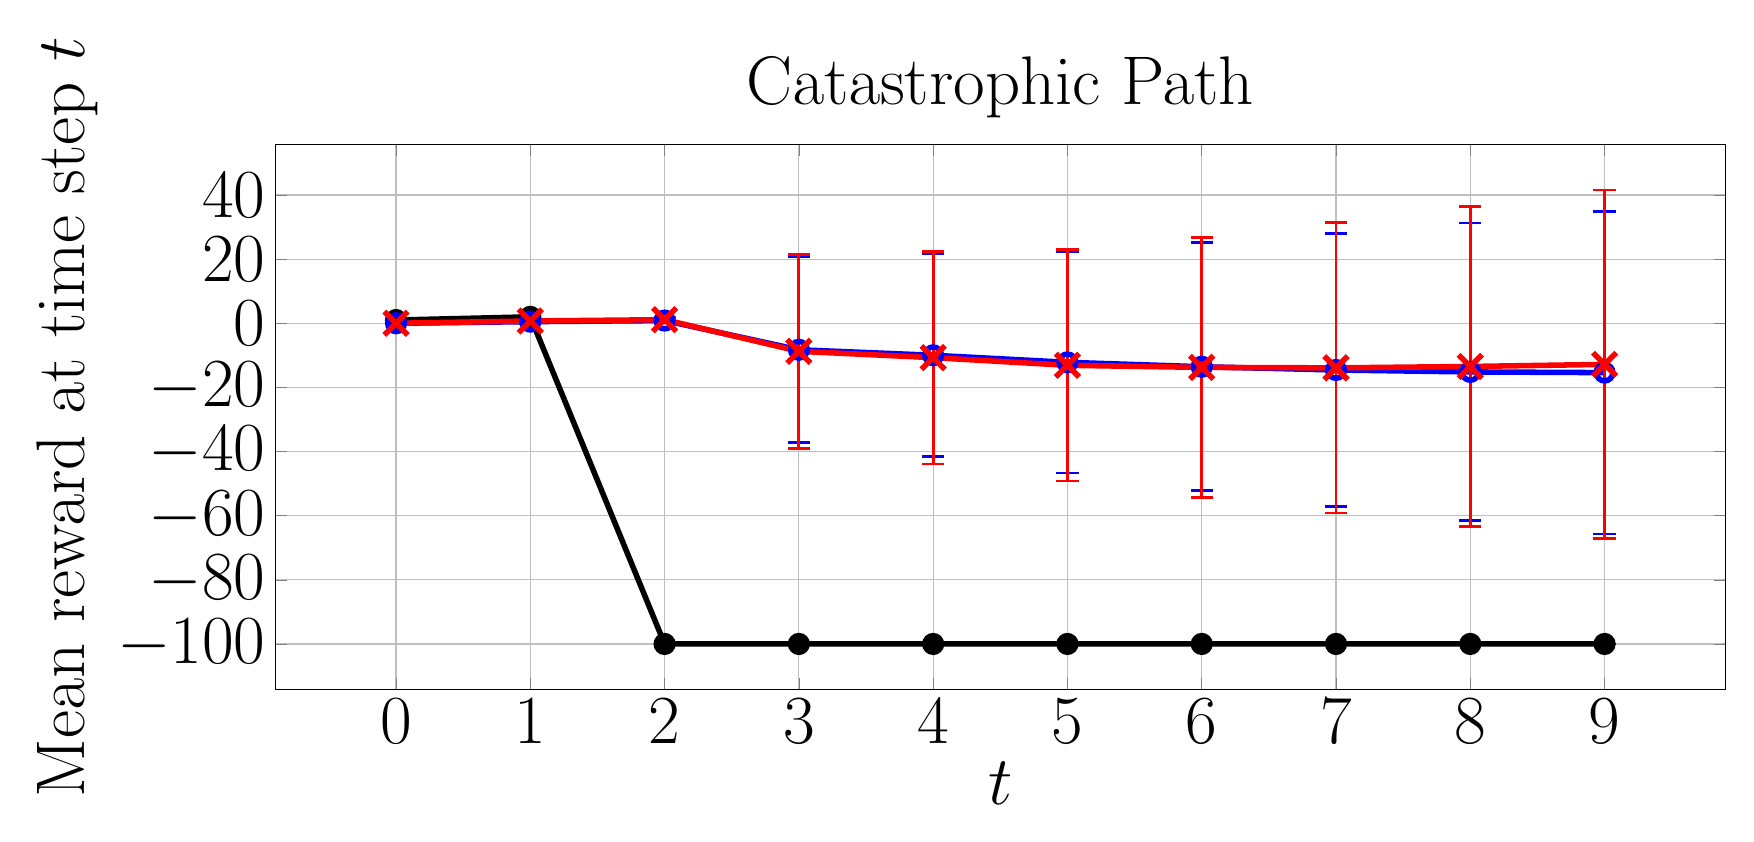
\begin{tikzpicture}
                \begin{axis}[
                    xlabel={$t$},
                    ylabel={Mean reward at time step $t$},
                    title={Catastrophic Path},
                    grid=both,
                    width=20cm, height=8.5cm,
                    every axis/.style={font=\Huge},
                    %
                ]
                \addplot[
                    color=black, %
                    mark=*, %
                    line width=2pt,
                    mark size=3pt,
                    error bars/.cd,
                    y dir=both, %
                    y explicit, %
                    error bar style={line width=1pt,solid},
                    error mark options={line width=1pt,mark size=4pt,rotate=90}
                ]
                coordinates {
                    (0, 1.0)  +- (0, 0.0)
                    (1, 2.0)  +- (0, 0.0) 
                    (2, -100.0)  +- (0, 0.0) 
                    (3, -100.0)  +- (0, 0.0)
                    (4, -100.0)  +- (0, 0.0)
                    (5, -100.0) +- (0, 0.0)
                    (6, -100.0) +- (0, 0.0)
                    (7, -100.0) +- (0, 0.0)
                    (8, -100.0) +- (0, 0.0)
                    (9, -100.0) +- (0, 0.0)
                };
                %
                \addplot[
                    color=blue, %
                    mark=o, %
                    line width=2pt,
                    mark size=3pt,
                    error bars/.cd,
                    y dir=both, %
                    y explicit, %
                    error bar style={line width=1pt,solid},
                    error mark options={line width=1pt,mark size=4pt,rotate=90}
                ]
                coordinates {
                    (0, 0.0)  +- (0, 0.0)
                    (1, 0.504814)  +- (0, 0.49997682) 
                    (2, 0.8439835)  +- (0, 0.76831917) 
                    (3, -8.2709165)  +- (0, 28.93656754)
                    (4, -9.981082)  +- (0, 31.66825363)
                    (5, -12.1776325) +- (0, 34.53463233)
                    (6, -13.556076) +- (0, 38.62845372)
                    (7, -14.574418) +- (0, 42.49603359)
                    (8, -15.1757075) +- (0, 46.41913968)
                    (9, -15.3900395) +- (0, 50.33563368)
                };
                %
                \addplot[
                    color=red, %
                    mark=x, %
                    line width=2pt,
                    mark size=6pt,
                    error bars/.cd,
                    y dir=both, %
                    y explicit, %
                    error bar style={line width=1pt,solid},
                    error mark options={line width=1pt,mark size=4pt,rotate=90}
                ]
                coordinates {
                    (0, 0.0)  +- (0, 0.0)
                    (1, 0.701873)  +- (0, 0.45743556) 
                    (2, 1.1227805)  +- (0, 0.73433129) 
                    (3, -8.7503255)  +- (0, 30.30257976)
                    (4, -10.722092)  +- (0, 33.17618589)
                    (5, -13.10721)  +- (0, 36.0648089)
                    (6, -13.7631645) +- (0, 40.56553451)
                    (7, -13.909043) +- (0, 45.23829402)
                    (8, -13.472517) +- (0, 49.96270296)
                    (9, -12.8278835) +- (0, 54.38618735)
                };
                %
            %
            %
            %
            %
            %
            %
            %
            %
            %
            %
            %
            %
            %
            %
            %
            %
            %
            %
                \end{axis}
            \end{tikzpicture}
         }
    }
    \caption{Average instant reward of CF paths induced by policies on GridWorld $p=0.4$.}
    \label{fig: reward p=0.4}
\end{figure*}

\subsection{Experimental Setup}
To compare policy performance, we measure the average rewards of counterfactual paths induced by our policy and the Gumbel-max policy by uniformly sampling $200$ counterfactual MDPs from the ICFMDP and generating $10,000$ counterfactual paths over each sampled CFMDP. \jl{Since the interval CFMDP depends on the observed path, we select $4$  paths of varying optimality to evaluate how the observed path impacts the performance of both policies: an optimal path, a slightly suboptimal path that could reach the optimal reward with a few changes, a catastrophic path that enters a catastrophic, terminal state with low reward, and an almost catastrophic path that was close to entering a catastrophic state.} When measuring the average probability bound widths and execution time needed to generate the ICFMDPs, we averaged over $20$ randomly generated observed paths
\footnote{Further training details are provided in Appendix \ref{app: training details}, and the code is provided at \href{https://github.com/ddv-lab/robust-cf-inference-in-MDPs}{https://github.com/ddv-lab/robust-cf-inference-in-MDPs}
%
%
.}.

\subsection{GridWorld}
\jl{The GridWorld MDP is a $4 \times 4$ grid where an agent must navigate from the top-left corner to the goal state in the bottom-right corner, avoiding a dangerous terminal state in the centre. At each time step, the agent can move up, down, left, or right, but there is a small probability (controlled by hyper-parameter $p$) of moving in an unintended direction. As the agent nears the goal, the reward for each state increases, culminating in a reward of $+100$ for reaching the goal. Entering the dangerous state results in a penalty of $-100$. We use two versions of GridWorld: a less stochastic version with $p=0.9$ (i.e., $90$\% chance of moving in the chosen direction) and a more stochastic version with $p=0.4$.}

\paragraph{GridWorld ($p=0.9$)}
When $p=0.9$, the counterfactual probability bounds are typically narrow (see Table \ref{tab:nonzero_probs} for average measurements). Consequently, as shown in Figure \ref{fig: reward p=0.9}, both policies are nearly identical and perform similarly well across the optimal, slightly suboptimal, and catastrophic paths.
%
However, for the almost catastrophic path, the interval CFMDP path is more conservative and follows the observed path more closely (as this is where the probability bounds are narrowest), which typically requires one additional step to reach the goal state than the Gumbel-max SCM policy.
%

\paragraph{GridWorld ($p=0.4$)}
\jl{When $p=0.4$, the GridWorld environment becomes more uncertain, increasing the risk of entering the dangerous state even if correct actions are chosen. Thus, as shown in Figure \ref{fig: reward p=0.4}, the interval CFMDP policy adopts a more conservative approach, avoiding deviation from the observed policy if it cannot guarantee higher counterfactual rewards (see the slightly suboptimal and almost catastrophic paths), whereas the Gumbel-max SCM is inconsistent: it can yield higher rewards, but also much lower rewards, reflected in the wide error bars.} For the catastrophic path, both policies must deviate from the observed path to achieve a higher reward and, in this case, perform similarly.
%
%
%
%
\subsection{Sepsis}
The Sepsis MDP \citep{oberst2019counterfactual} simulates trajectories of Sepsis patients. Each state consists of four vital signs (heart rate, blood pressure, oxygen concentration, and glucose levels), categorised as low, normal, or high.
and three treatments that can be toggled on/off at each time step (8 actions in total). Unlike \citet{oberst2019counterfactual}, we scale rewards based on the number of out-of-range vital signs, between $-1000$ (patient dies) and $1000$ (patient discharged). \jl{Like the GridWorld $p=0.4$ experiment, the Sepsis MDP is highly uncertain, as many states are equally likely to lead to optimal and poor outcomes. Thus, as shown in Figure \ref{fig: reward sepsis}, both policies follow the observed optimal and almost catastrophic paths to guarantee rewards are no worse than the observation.} However, improving the catastrophic path requires deviating from the observation. Here, the Gumbel-max SCM policy, on average, performs better than the interval CFMDP policy. But, since both policies have lower bounds clipped at $-1000$, neither policy reliably improves over the observation. In contrast, for the slightly suboptimal path, the interval CFMDP policy performs significantly better, shown by its higher lower bounds. 
Moreover, in these two cases, the worst-case counterfactual path generated by the interval CFMDP policy is better than that of the Gumbel-max SCM policy,
indicating its greater robustness.
%
\begin{figure*}
    \centering
     \resizebox{0.6\textwidth}{!}{
        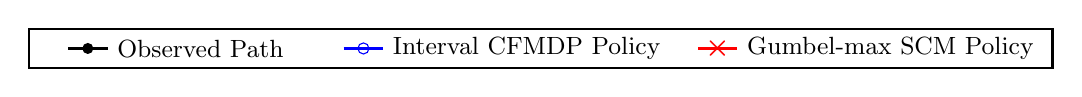
\begin{tikzpicture}[scale=1.0, every node/.style={scale=1.0}]
            \draw[thick, black] (-3, -0.25) rectangle (10, 0.25);
            %
            \draw[black, line width=1pt] (-2.5, 0.0) -- (-2,0.0);
            \fill[black] (-2.25,0.0) circle (2pt); %
            \node[right] at (-2,0.0) {\small Observed Path};
            
            %
            \draw[blue, line width=1pt] (1.0,0.0) -- (1.5,0.0);
            \node[draw=blue, circle, minimum size=4pt, inner sep=0pt] at (1.25,0.0) {}; %
            \node[right] at (1.5,0.0) {\small Interval CFMDP Policy};
            
            %
            \draw[red, line width=1pt] (5.5,0) -- (6,0);
            \node[red] at (5.75,0) {$\boldsymbol{\times}$}; %
            \node[right] at (6,0) {\small Gumbel-max SCM Policy};
        \end{tikzpicture}
    }\\
    \subfigure[\footnotesize Lowest cumulative reward: Interval CFMDP ($8000$), Gumbel-max SCM ($8000$)]{%
         \resizebox{0.76\columnwidth}{!}{
             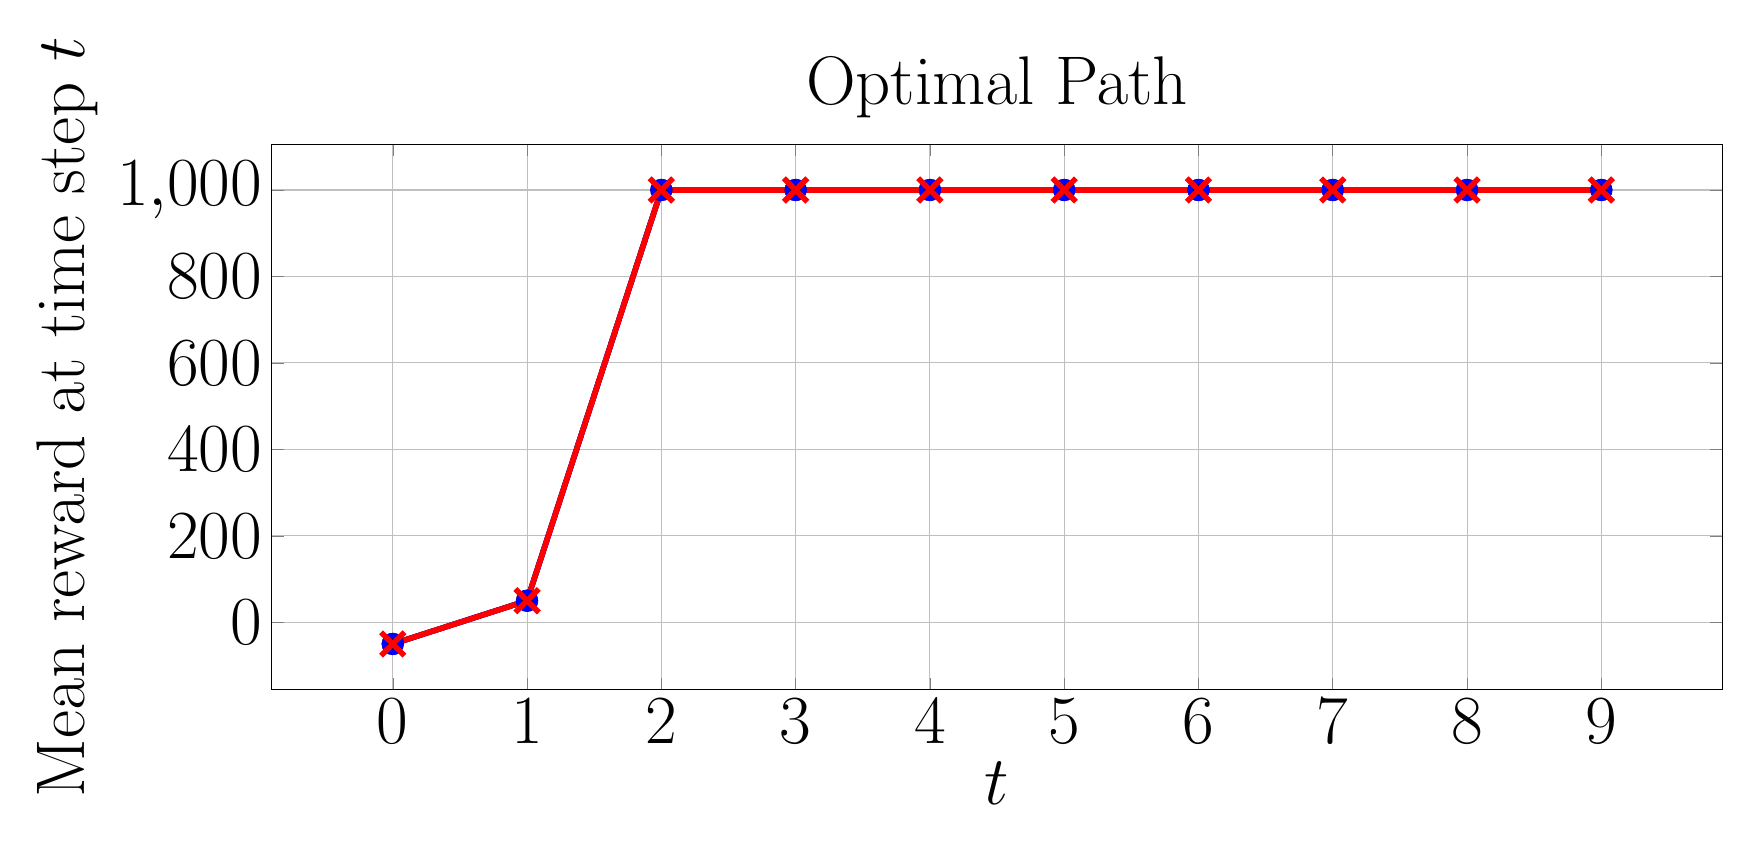
\begin{tikzpicture}
                \begin{axis}[
                    xlabel={$t$},
                    ylabel={Mean reward at time step $t$},
                    title={Optimal Path},
                    grid=both,
                    width=20cm, height=8.5cm,
                    every axis/.style={font=\Huge},
                    %
                ]
                \addplot[
                    color=black, %
                    mark=*, %
                    line width=2pt,
                    mark size=3pt,
                ]
                coordinates {
                    (0, -50.0)
                    (1, 50.0)
                    (2, 1000.0)
                    (3, 1000.0)
                    (4, 1000.0)
                    (5, 1000.0)
                    (6, 1000.0)
                    (7, 1000.0)
                    (8, 1000.0)
                    (9, 1000.0)
                };
                %
                \addplot[
                    color=blue, %
                    mark=o, %
                    line width=2pt,
                    mark size=3pt,
                    error bars/.cd,
                    y dir=both, %
                    y explicit, %
                    error bar style={line width=1pt,solid},
                    error mark options={line width=1pt,mark size=4pt,rotate=90}
                ]
                coordinates {
                    (0, -50.0)  +- (0, 0.0)
                    (1, 50.0)  +- (0, 0.0) 
                    (2, 1000.0)  +- (0, 0.0) 
                    (3, 1000.0)  +- (0, 0.0)
                    (4, 1000.0)  +- (0, 0.0)
                    (5, 1000.0) +- (0, 0.0)
                    (6, 1000.0) +- (0, 0.0)
                    (7, 1000.0) +- (0, 0.0)
                    (8, 1000.0) +- (0, 0.0)
                    (9, 1000.0) +- (0, 0.0)
                };
                %
                \addplot[
                    color=red, %
                    mark=x, %
                    line width=2pt,
                    mark size=6pt,
                    error bars/.cd,
                    y dir=both, %
                    y explicit, %
                    error bar style={line width=1pt,solid},
                    error mark options={line width=1pt,mark size=4pt,rotate=90}
                ]
                coordinates {
                    (0, -50.0)  +- (0, 0.0)
                    (1, 50.0)  +- (0, 0.0) 
                    (2, 1000.0)  +- (0, 0.0) 
                    (3, 1000.0)  +- (0, 0.0)
                    (4, 1000.0)  +- (0, 0.0)
                    (5, 1000.0) +- (0, 0.0)
                    (6, 1000.0) +- (0, 0.0)
                    (7, 1000.0) +- (0, 0.0)
                    (8, 1000.0) +- (0, 0.0)
                    (9, 1000.0) +- (0, 0.0)
                };
                %
                \end{axis}
            \end{tikzpicture}
         }
    }
    \hspace{1cm}
    \subfigure[\footnotesize Lowest cumulative reward: Interval CFMDP ($-5980$), Gumbel-max SCM ($-8000$)]{%
         \resizebox{0.76\columnwidth}{!}{
            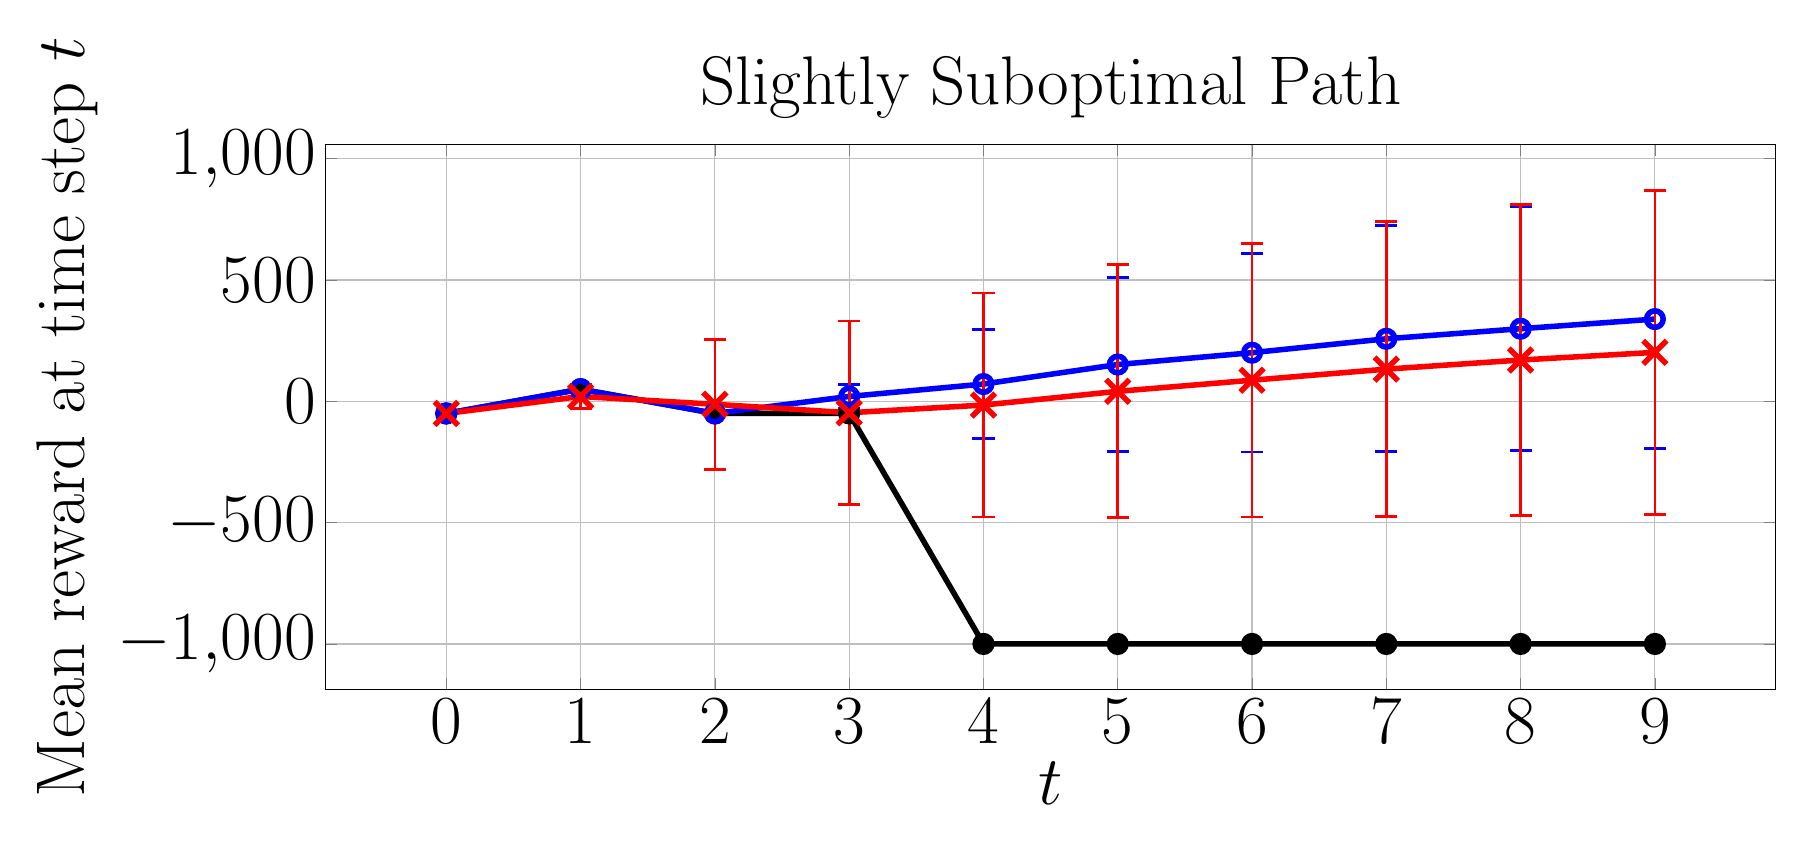
\begin{tikzpicture}
                \begin{axis}[
                    xlabel={$t$},
                    ylabel={Mean reward at time step $t$},
                    title={Slightly Suboptimal Path},
                    grid=both,
                    width=20cm, height=8.5cm,
                    every axis/.style={font=\Huge},
                    %
                ]
               \addplot[
                    color=black, %
                    mark=*, %
                    line width=2pt,
                    mark size=3pt,
                ]
                coordinates {
                    (0, -50.0)
                    (1, 50.0)
                    (2, -50.0)
                    (3, -50.0)
                    (4, -1000.0)
                    (5, -1000.0)
                    (6, -1000.0)
                    (7, -1000.0)
                    (8, -1000.0)
                    (9, -1000.0)
                };
                %
                \addplot[
                    color=blue, %
                    mark=o, %
                    line width=2pt,
                    mark size=3pt,
                    error bars/.cd,
                    y dir=both, %
                    y explicit, %
                    error bar style={line width=1pt,solid},
                    error mark options={line width=1pt,mark size=4pt,rotate=90}
                ]
                coordinates {
                    (0, -50.0)  +- (0, 0.0)
                    (1, 50.0)  +- (0, 0.0) 
                    (2, -50.0)  +- (0, 0.0) 
                    (3, 20.0631)  +- (0, 49.97539413)
                    (4, 71.206585)  +- (0, 226.02033693)
                    (5, 151.60797) +- (0, 359.23292559)
                    (6, 200.40593) +- (0, 408.86185176)
                    (7, 257.77948) +- (0, 466.10372804)
                    (8, 299.237465) +- (0, 501.82579506)
                    (9, 338.9129) +- (0, 532.06124996)
                };
                %
                \addplot[
                    color=red, %
                    mark=x, %
                    line width=2pt,
                    mark size=6pt,
                    error bars/.cd,
                    y dir=both, %
                    y explicit, %
                    error bar style={line width=1pt,solid},
                    error mark options={line width=1pt,mark size=4pt,rotate=90}
                ]
                coordinates {
                    (0, -50.0)  +- (0, 0.0)
                    (1, 20.00736)  +- (0, 49.99786741) 
                    (2, -12.282865)  +- (0, 267.598755) 
                    (3, -47.125995)  +- (0, 378.41755832)
                    (4, -15.381965)  +- (0, 461.77616558)
                    (5, 41.15459) +- (0, 521.53189262)
                    (6, 87.01595) +- (0, 564.22243126 )
                    (7, 132.62376) +- (0, 607.31338037)
                    (8, 170.168145) +- (0, 641.48013693)
                    (9, 201.813135) +- (0, 667.29441777)
                };
                %
                %
                %
                %
                %
                %
                %
                %
                %
                %
                %
                %
                %
                %
                %
                %
                %
                %
                %
                \end{axis}
            \end{tikzpicture}
         }
    }\\[-1.5pt]
    \subfigure[\footnotesize Lowest cumulative reward: Interval CFMDP ($100$), Gumbel-max SCM ($100$)]{%
         \resizebox{0.76\columnwidth}{!}{
             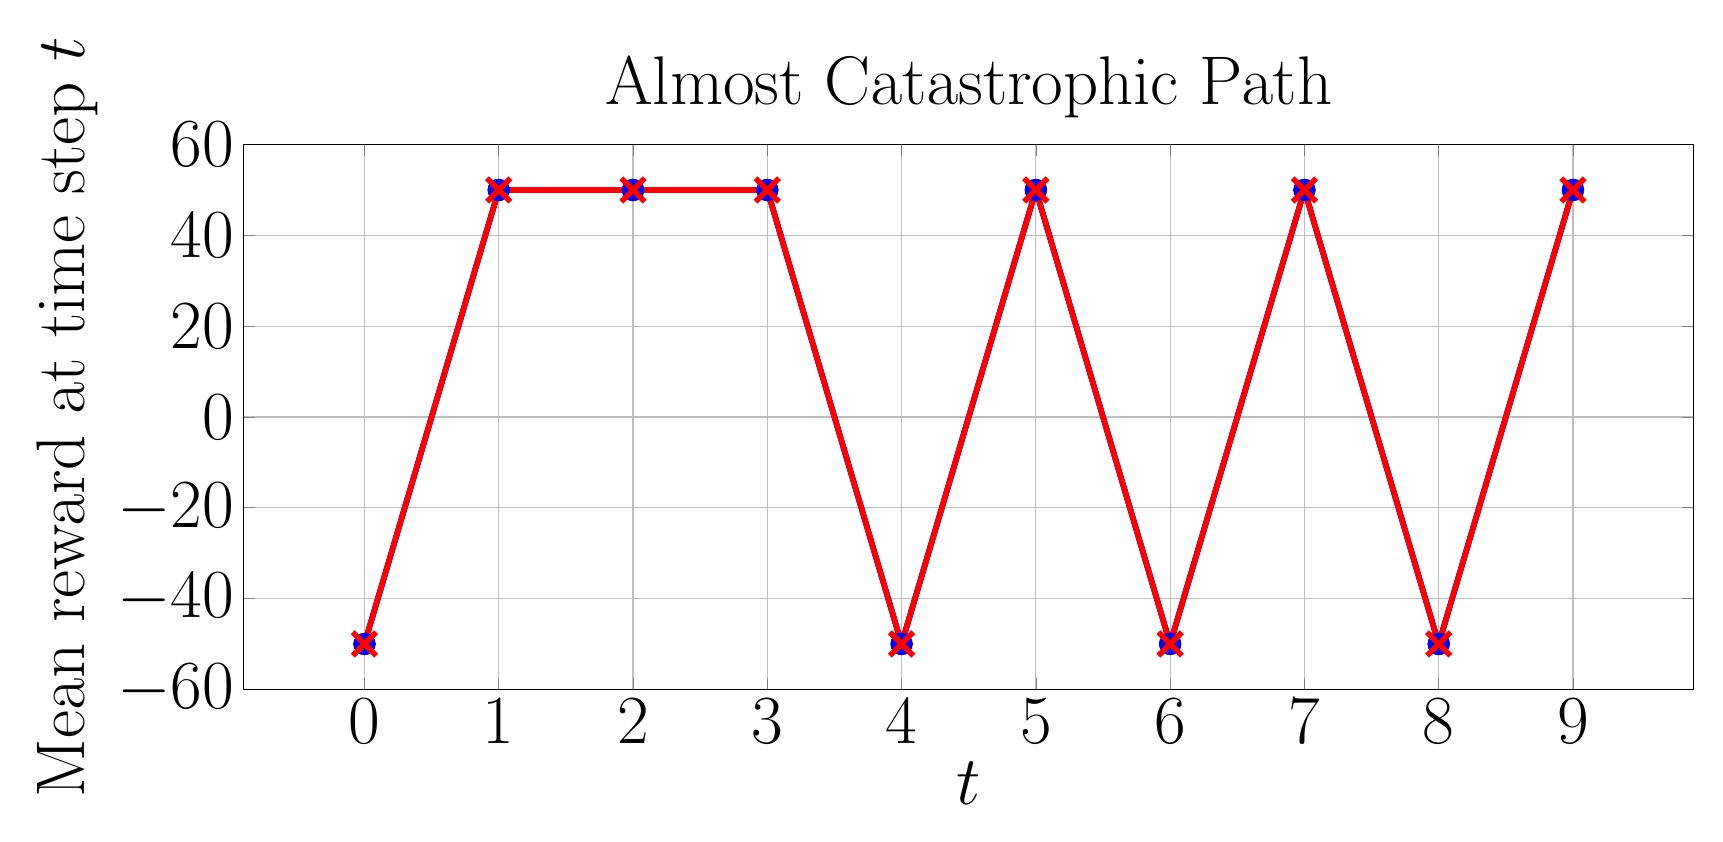
\begin{tikzpicture}
                \begin{axis}[
                    xlabel={$t$},
                    ylabel={Mean reward at time step $t$},
                    title={Almost Catastrophic Path},
                    grid=both,
                    every axis/.style={font=\Huge},
                    width=20cm, height=8.5cm,
                    %
                ]
               \addplot[
                    color=black, %
                    mark=*, %
                    line width=2pt,
                    mark size=3pt,
                ]
                coordinates {
                    (0, -50.0)
                    (1, 50.0)
                    (2, 50.0)
                    (3, 50.0)
                    (4, -50.0)
                    (5, 50.0)
                    (6, -50.0)
                    (7, 50.0)
                    (8, -50.0)
                    (9, 50.0)
                };
                %
                %
                \addplot[
                    color=blue, %
                    mark=o, %
                    line width=2pt,
                    mark size=3pt,
                    error bars/.cd,
                    y dir=both, %
                    y explicit, %
                    error bar style={line width=1pt,solid},
                    error mark options={line width=1pt,mark size=4pt,rotate=90}
                ]
                coordinates {
                    (0, -50.0)  +- (0, 0.0)
                    (1, 50.0)  +- (0, 0.0) 
                    (2, 50.0)  +- (0, 0.0) 
                    (3, 50.0)  +- (0, 0.0)
                    (4, -50.0)  +- (0, 0.0)
                    (5, 50.0) +- (0, 0.0)
                    (6, -50.0) +- (0, 0.0)
                    (7, 50.0) +- (0, 0.0)
                    (8, -50.0) +- (0, 0.0)
                    (9, 50.0) +- (0, 0.0)
                };
                %
                \addplot[
                    color=red, %
                    mark=x, %
                    line width=2pt,
                    mark size=6pt,
                    error bars/.cd,
                    y dir=both, %
                    y explicit, %
                    error bar style={line width=1pt,solid},
                    error mark options={line width=1pt,mark size=4pt,rotate=90}
                ]
                coordinates {
                    (0, -50.0)  +- (0, 0.0)
                    (1, 50.0)  +- (0, 0.0) 
                    (2, 50.0)  +- (0, 0.0) 
                    (3, 50.0)  +- (0, 0.0)
                    (4, -50.0)  +- (0, 0.0)
                    (5, 50.0) +- (0, 0.0)
                    (6, -50.0) +- (0, 0.0)
                    (7, 50.0) +- (0, 0.0)
                    (8, -50.0) +- (0, 0.0)
                    (9, 50.0) +- (0, 0.0)
                };
                %
                %
                %
                %
                %
                %
                %
                %
                %
                %
                %
                %
                %
                %
                %
                %
                %
                %
                %
                \end{axis}
            \end{tikzpicture}
         }
    }
    \hspace{1cm}
    \subfigure[\footnotesize Lowest cumulative reward: Interval CFMDP ($-7150$), Gumbel-max SCM ($-9050$)]{%
         \resizebox{0.76\columnwidth}{!}{
            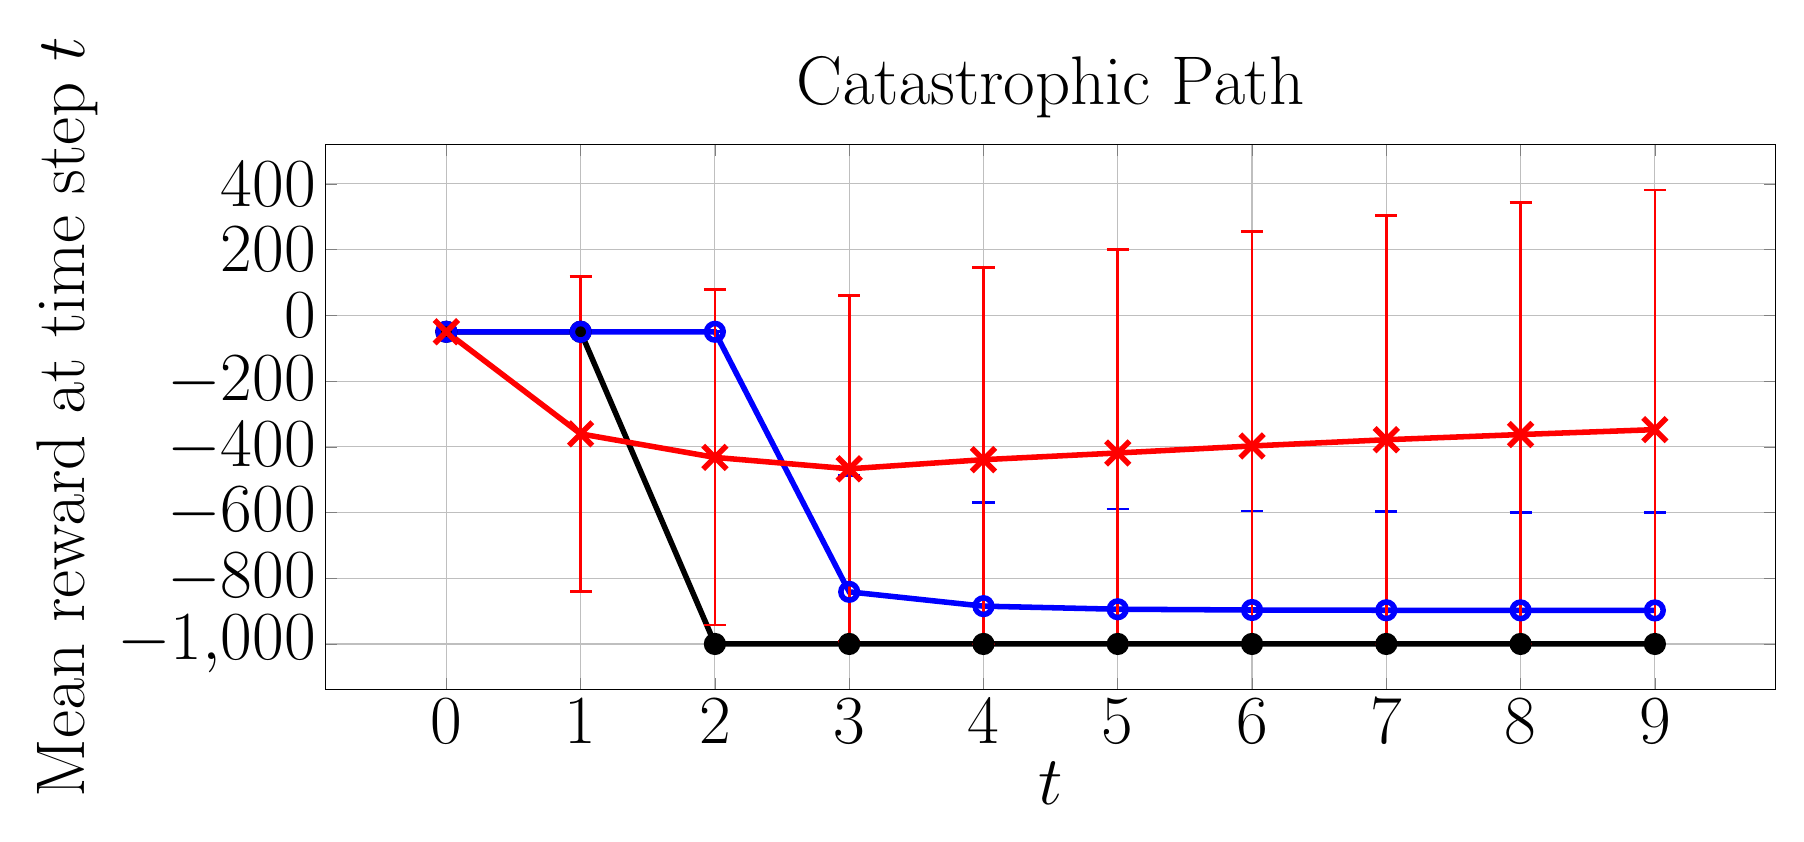
\begin{tikzpicture}
                \begin{axis}[
                    xlabel={$t$},
                    ylabel={Mean reward at time step $t$},
                    title={Catastrophic Path},
                    grid=both,
                    width=20cm, height=8.5cm,
                    every axis/.style={font=\Huge},
                    %
                ]
               \addplot[
                    color=black, %
                    mark=*, %
                    line width=2pt,
                    mark size=3pt,
                ]
                coordinates {
                    (0, -50.0)
                    (1, -50.0)
                    (2, -1000.0)
                    (3, -1000.0)
                    (4, -1000.0)
                    (5, -1000.0)
                    (6, -1000.0)
                    (7, -1000.0)
                    (8, -1000.0)
                    (9, -1000.0)
                };
                %
                %
                \addplot[
                    color=blue, %
                    mark=o, %
                    line width=2pt,
                    mark size=3pt,
                    error bars/.cd,
                    y dir=both, %
                    y explicit, %
                    error bar style={line width=1pt,solid},
                    error mark options={line width=1pt,mark size=4pt,rotate=90}
                ]
                coordinates {
                    (0, -50.0)  +- (0, 0.0)
                    (1, -50.0)  +- (0, 0.0) 
                    (2, -50.0)  +- (0, 0.0) 
                    (3, -841.440725)  += (0, 354.24605512) -= (0, 158.559275)
                    (4, -884.98225)  += (0, 315.37519669) -= (0, 115.01775)
                    (5, -894.330425) += (0, 304.88572805) -= (0, 105.669575)
                    (6, -896.696175) += (0, 301.19954514) -= (0, 103.303825)
                    (7, -897.4635) += (0, 299.61791279) -= (0, 102.5365)
                    (8, -897.77595) += (0, 298.80392585) -= (0, 102.22405)
                    (9, -897.942975) += (0, 298.32920557) -= (0, 102.057025)
                };
                %
                \addplot[
                    color=red, %
                    mark=x, %
                    line width=2pt,
                    mark size=6pt,
                    error bars/.cd,
                    y dir=both, %
                    y explicit, %
                    error bar style={line width=1pt,solid},
                    error mark options={line width=1pt,mark size=4pt,rotate=90}
                ]
            coordinates {
                    (0, -50.0)  +- (0, 0.0)
                    (1, -360.675265)  +- (0, 479.39812699) 
                    (2, -432.27629)  +- (0, 510.38620897) 
                    (3, -467.029545)  += (0, 526.36009628) -= (0, 526.36009628)
                    (4, -439.17429)  += (0, 583.96638919) -= (0, 560.82571)
                    (5, -418.82704) += (0, 618.43027478) -= (0, 581.17296)
                    (6, -397.464895) += (0, 652.67322574) -= (0, 602.535105)
                    (7, -378.49052) += (0, 682.85407033) -= (0, 621.50948)
                    (8, -362.654195) += (0, 707.01412023) -= (0, 637.345805)
                    (9, -347.737935) += (0, 729.29076479) -= (0, 652.262065)
                };
                %
                %
                %
                %
                %
                %
                %
                %
                %
                %
                %
                %
                %
                %
                %
                %
                %
                %
                %
                \end{axis}
            \end{tikzpicture}
         }
    }
    \caption{Average instant reward of CF paths induced by policies on Sepsis.}
    \label{fig: reward sepsis}
\end{figure*}

%
%
%
\subsection{Interval CFMDP Bounds}
%
%
Table \ref{tab:nonzero_probs} presents the mean counterfactual probability bound widths (excluding transitions where the upper bound is $0$) for each MDP, averaged over 20 observed paths. We compare the bounds under counterfactual stability (CS) and monotonicity (M) assumptions, CS alone, and no assumptions. This shows that the assumptions marginally reduce the bound widths, indicating the assumptions tighten the bounds without excluding too many causal models, as intended.
\renewcommand{\arraystretch}{1}

\begin{table}
\centering
\caption{Mean width of counterfactual probability bounds}
\resizebox{0.8\columnwidth}{!}{%
\begin{tabular}{|c|c|c|c|}
\hline
\multirow{2}{*}{\textbf{Environment}} & \multicolumn{3}{c|}{\textbf{Assumptions}} \\ \cline{2-4}
 & \textbf{CS + M} & \textbf{CS} & \textbf{None\tablefootnote{\jl{Equivalent to \citet{li2024probabilities}'s bounds (see Section \ref{sec: equivalence with Li}).}}} \\ \hline
\textbf{GridWorld} ($p=0.9$) & 0.0817 & 0.0977 & 0.100 \\ \hline
\textbf{GridWorld} ($p=0.4$) & 0.552  & 0.638  & 0.646 \\ \hline
\textbf{Sepsis} & 0.138 & 0.140 & 0.140 \\ \hline
\end{tabular}
}
\label{tab:nonzero_probs}
\end{table}


\subsection{Execution Times}
Table \ref{tab: times} compares the average time needed to generate the interval CFMDP vs.\ the Gumbel-max SCM CFMDP for 20 observations.
The GridWorld algorithms were run single-threaded, while the Sepsis experiments were run in parallel.
Generating the interval CFMDP is significantly faster as it uses exact analytical bounds, whereas the Gumbel-max CFMDP requires sampling from the Gumbel distribution to estimate counterfactual transition probabilities. \jl{Since constructing the counterfactual MDP models is the main bottleneck in both approaches, ours is more efficient overall and suitable for larger MDPs.}
\begin{table}
\centering
\caption{Mean execution time to generate CFMDPs}
\resizebox{0.99\columnwidth}{!}{%
\begin{tabular}{|c|c|c|}
\hline
\multirow{2}{*}{\textbf{Environment}} & \multicolumn{2}{c|}{\textbf{Mean Execution Time (s)}} \\ \cline{2-3} 
                                      & \textbf{Interval CFMDP} & \textbf{Gumbel-max CFMDP} \\ \hline
\textbf{GridWorld ($p=0.9$) }                  & 0.261                   & 56.1                      \\ \hline
\textbf{GridWorld ($p=0.4$)  }                 & 0.336                   & 54.5                      \\ \hline
\textbf{Sepsis}                                 & 688                     & 2940                      \\ \hline
\end{tabular}%
}
\label{tab: times}
\end{table}


\begin{table*}[t]
\centering
\fontsize{11pt}{11pt}\selectfont
\begin{tabular}{lllllllllllll}
\toprule
\multicolumn{1}{c}{\textbf{task}} & \multicolumn{2}{c}{\textbf{Mir}} & \multicolumn{2}{c}{\textbf{Lai}} & \multicolumn{2}{c}{\textbf{Ziegen.}} & \multicolumn{2}{c}{\textbf{Cao}} & \multicolumn{2}{c}{\textbf{Alva-Man.}} & \multicolumn{1}{c}{\textbf{avg.}} & \textbf{\begin{tabular}[c]{@{}l@{}}avg.\\ rank\end{tabular}} \\
\multicolumn{1}{c}{\textbf{metrics}} & \multicolumn{1}{c}{\textbf{cor.}} & \multicolumn{1}{c}{\textbf{p-v.}} & \multicolumn{1}{c}{\textbf{cor.}} & \multicolumn{1}{c}{\textbf{p-v.}} & \multicolumn{1}{c}{\textbf{cor.}} & \multicolumn{1}{c}{\textbf{p-v.}} & \multicolumn{1}{c}{\textbf{cor.}} & \multicolumn{1}{c}{\textbf{p-v.}} & \multicolumn{1}{c}{\textbf{cor.}} & \multicolumn{1}{c}{\textbf{p-v.}} &  &  \\ \midrule
\textbf{S-Bleu} & 0.50 & 0.0 & 0.47 & 0.0 & 0.59 & 0.0 & 0.58 & 0.0 & 0.68 & 0.0 & 0.57 & 5.8 \\
\textbf{R-Bleu} & -- & -- & 0.27 & 0.0 & 0.30 & 0.0 & -- & -- & -- & -- & - &  \\
\textbf{S-Meteor} & 0.49 & 0.0 & 0.48 & 0.0 & 0.61 & 0.0 & 0.57 & 0.0 & 0.64 & 0.0 & 0.56 & 6.1 \\
\textbf{R-Meteor} & -- & -- & 0.34 & 0.0 & 0.26 & 0.0 & -- & -- & -- & -- & - &  \\
\textbf{S-Bertscore} & \textbf{0.53} & 0.0 & {\ul 0.80} & 0.0 & \textbf{0.70} & 0.0 & {\ul 0.66} & 0.0 & {\ul0.78} & 0.0 & \textbf{0.69} & \textbf{1.7} \\
\textbf{R-Bertscore} & -- & -- & 0.51 & 0.0 & 0.38 & 0.0 & -- & -- & -- & -- & - &  \\
\textbf{S-Bleurt} & {\ul 0.52} & 0.0 & {\ul 0.80} & 0.0 & 0.60 & 0.0 & \textbf{0.70} & 0.0 & \textbf{0.80} & 0.0 & {\ul 0.68} & {\ul 2.3} \\
\textbf{R-Bleurt} & -- & -- & 0.59 & 0.0 & -0.05 & 0.13 & -- & -- & -- & -- & - &  \\
\textbf{S-Cosine} & 0.51 & 0.0 & 0.69 & 0.0 & {\ul 0.62} & 0.0 & 0.61 & 0.0 & 0.65 & 0.0 & 0.62 & 4.4 \\
\textbf{R-Cosine} & -- & -- & 0.40 & 0.0 & 0.29 & 0.0 & -- & -- & -- & -- & - & \\ \midrule
\textbf{QuestEval} & 0.23 & 0.0 & 0.25 & 0.0 & 0.49 & 0.0 & 0.47 & 0.0 & 0.62 & 0.0 & 0.41 & 9.0 \\
\textbf{LLaMa3} & 0.36 & 0.0 & \textbf{0.84} & 0.0 & {\ul{0.62}} & 0.0 & 0.61 & 0.0 &  0.76 & 0.0 & 0.64 & 3.6 \\
\textbf{our (3b)} & 0.49 & 0.0 & 0.73 & 0.0 & 0.54 & 0.0 & 0.53 & 0.0 & 0.7 & 0.0 & 0.60 & 5.8 \\
\textbf{our (8b)} & 0.48 & 0.0 & 0.73 & 0.0 & 0.52 & 0.0 & 0.53 & 0.0 & 0.7 & 0.0 & 0.59 & 6.3 \\  \bottomrule
\end{tabular}
\caption{Pearson correlation on human evaluation on system output. `R-': reference-based. `S-': source-based.}
\label{tab:sys}
\end{table*}



\begin{table}%[]
\centering
\fontsize{11pt}{11pt}\selectfont
\begin{tabular}{llllll}
\toprule
\multicolumn{1}{c}{\textbf{task}} & \multicolumn{1}{c}{\textbf{Lai}} & \multicolumn{1}{c}{\textbf{Zei.}} & \multicolumn{1}{c}{\textbf{Scia.}} & \textbf{} & \textbf{} \\ 
\multicolumn{1}{c}{\textbf{metrics}} & \multicolumn{1}{c}{\textbf{cor.}} & \multicolumn{1}{c}{\textbf{cor.}} & \multicolumn{1}{c}{\textbf{cor.}} & \textbf{avg.} & \textbf{\begin{tabular}[c]{@{}l@{}}avg.\\ rank\end{tabular}} \\ \midrule
\textbf{S-Bleu} & 0.40 & 0.40 & 0.19* & 0.33 & 7.67 \\
\textbf{S-Meteor} & 0.41 & 0.42 & 0.16* & 0.33 & 7.33 \\
\textbf{S-BertS.} & {\ul0.58} & 0.47 & 0.31 & 0.45 & 3.67 \\
\textbf{S-Bleurt} & 0.45 & {\ul 0.54} & {\ul 0.37} & 0.45 & {\ul 3.33} \\
\textbf{S-Cosine} & 0.56 & 0.52 & 0.3 & {\ul 0.46} & {\ul 3.33} \\ \midrule
\textbf{QuestE.} & 0.27 & 0.35 & 0.06* & 0.23 & 9.00 \\
\textbf{LlaMA3} & \textbf{0.6} & \textbf{0.67} & \textbf{0.51} & \textbf{0.59} & \textbf{1.0} \\
\textbf{Our (3b)} & 0.51 & 0.49 & 0.23* & 0.39 & 4.83 \\
\textbf{Our (8b)} & 0.52 & 0.49 & 0.22* & 0.43 & 4.83 \\ \bottomrule
\end{tabular}
\caption{Pearson correlation on human ratings on reference output. *not significant; we cannot reject the null hypothesis of zero correlation}
\label{tab:ref}
\end{table}


\begin{table*}%[]
\centering
\fontsize{11pt}{11pt}\selectfont
\begin{tabular}{lllllllll}
\toprule
\textbf{task} & \multicolumn{1}{c}{\textbf{ALL}} & \multicolumn{1}{c}{\textbf{sentiment}} & \multicolumn{1}{c}{\textbf{detoxify}} & \multicolumn{1}{c}{\textbf{catchy}} & \multicolumn{1}{c}{\textbf{polite}} & \multicolumn{1}{c}{\textbf{persuasive}} & \multicolumn{1}{c}{\textbf{formal}} & \textbf{\begin{tabular}[c]{@{}l@{}}avg. \\ rank\end{tabular}} \\
\textbf{metrics} & \multicolumn{1}{c}{\textbf{cor.}} & \multicolumn{1}{c}{\textbf{cor.}} & \multicolumn{1}{c}{\textbf{cor.}} & \multicolumn{1}{c}{\textbf{cor.}} & \multicolumn{1}{c}{\textbf{cor.}} & \multicolumn{1}{c}{\textbf{cor.}} & \multicolumn{1}{c}{\textbf{cor.}} &  \\ \midrule
\textbf{S-Bleu} & -0.17 & -0.82 & -0.45 & -0.12* & -0.1* & -0.05 & -0.21 & 8.42 \\
\textbf{R-Bleu} & - & -0.5 & -0.45 &  &  &  &  &  \\
\textbf{S-Meteor} & -0.07* & -0.55 & -0.4 & -0.01* & 0.1* & -0.16 & -0.04* & 7.67 \\
\textbf{R-Meteor} & - & -0.17* & -0.39 & - & - & - & - & - \\
\textbf{S-BertScore} & 0.11 & -0.38 & -0.07* & -0.17* & 0.28 & 0.12 & 0.25 & 6.0 \\
\textbf{R-BertScore} & - & -0.02* & -0.21* & - & - & - & - & - \\
\textbf{S-Bleurt} & 0.29 & 0.05* & 0.45 & 0.06* & 0.29 & 0.23 & 0.46 & 4.2 \\
\textbf{R-Bleurt} & - &  0.21 & 0.38 & - & - & - & - & - \\
\textbf{S-Cosine} & 0.01* & -0.5 & -0.13* & -0.19* & 0.05* & -0.05* & 0.15* & 7.42 \\
\textbf{R-Cosine} & - & -0.11* & -0.16* & - & - & - & - & - \\ \midrule
\textbf{QuestEval} & 0.21 & {\ul{0.29}} & 0.23 & 0.37 & 0.19* & 0.35 & 0.14* & 4.67 \\
\textbf{LlaMA3} & \textbf{0.82} & \textbf{0.80} & \textbf{0.72} & \textbf{0.84} & \textbf{0.84} & \textbf{0.90} & \textbf{0.88} & \textbf{1.00} \\
\textbf{Our (3b)} & 0.47 & -0.11* & 0.37 & 0.61 & 0.53 & 0.54 & 0.66 & 3.5 \\
\textbf{Our (8b)} & {\ul{0.57}} & 0.09* & {\ul 0.49} & {\ul 0.72} & {\ul 0.64} & {\ul 0.62} & {\ul 0.67} & {\ul 2.17} \\ \bottomrule
\end{tabular}
\caption{Pearson correlation on human ratings on our constructed test set. 'R-': reference-based. 'S-': source-based. *not significant; we cannot reject the null hypothesis of zero correlation}
\label{tab:con}
\end{table*}

\section{Results}
We benchmark the different metrics on the different datasets using correlation to human judgement. For content preservation, we show results split on data with system output, reference output and our constructed test set: we show that the data source for evaluation leads to different conclusions on the metrics. In addition, we examine whether the metrics can rank style transfer systems similar to humans. On style strength, we likewise show correlations between human judgment and zero-shot evaluation approaches. When applicable, we summarize results by reporting the average correlation. And the average ranking of the metric per dataset (by ranking which metric obtains the highest correlation to human judgement per dataset). 

\subsection{Content preservation}
\paragraph{How do data sources affect the conclusion on best metric?}
The conclusions about the metrics' performance change radically depending on whether we use system output data, reference output, or our constructed test set. Ideally, a good metric correlates highly with humans on any data source. Ideally, for meta-evaluation, a metric should correlate consistently across all data sources, but the following shows that the correlations indicate different things, and the conclusion on the best metric should be drawn carefully.

Looking at the metrics correlations with humans on the data source with system output (Table~\ref{tab:sys}), we see a relatively high correlation for many of the metrics on many tasks. The overall best metrics are S-BertScore and S-BLEURT (avg+avg rank). We see no notable difference in our method of using the 3B or 8B model as the backbone.

Examining the average correlations based on data with reference output (Table~\ref{tab:ref}), now the zero-shoot prompting with LlaMA3 70B is the best-performing approach ($0.59$ avg). Tied for second place are source-based cosine embedding ($0.46$ avg), BLEURT ($0.45$ avg) and BertScore ($0.45$ avg). Our method follows on a 5. place: here, the 8b version (($0.43$ avg)) shows a bit stronger results than 3b ($0.39$ avg). The fact that the conclusions change, whether looking at reference or system output, confirms the observations made by \citet{scialom-etal-2021-questeval} on simplicity transfer.   

Now consider the results on our test set (Table~\ref{tab:con}): Several metrics show low or no correlation; we even see a significantly negative correlation for some metrics on ALL (BLEU) and for specific subparts of our test set for BLEU, Meteor, BertScore, Cosine. On the other end, LlaMA3 70B is again performing best, showing strong results ($0.82$ in ALL). The runner-up is now our 8B method, with a gap to the 3B version ($0.57$ vs $0.47$ in ALL). Note our method still shows zero correlation for the sentiment task. After, ranks BLEURT ($0.29$), QuestEval ($0.21$), BertScore ($0.11$), Cosine ($0.01$).  

On our test set, we find that some metrics that correlate relatively well on the other datasets, now exhibit low correlation. Hence, with our test set, we can now support the logical reasoning with data evidence: Evaluation of content preservation for style transfer needs to take the style shift into account. This conclusion could not be drawn using the existing data sources: We hypothesise that for the data with system-based output, successful output happens to be very similar to the source sentence and vice versa, and reference-based output might not contain server mistakes as they are gold references. Thus, none of the existing data sources tests the limits of the metrics.  


\paragraph{How do reference-based metrics compare to source-based ones?} Reference-based metrics show a lower correlation than the source-based counterpart for all metrics on both datasets with ratings on references (Table~\ref{tab:sys}). As discussed previously, reference-based metrics for style transfer have the drawback that many different good solutions on a rewrite might exist and not only one similar to a reference.


\paragraph{How well can the metrics rank the performance of style transfer methods?}
We compare the metrics' ability to judge the best style transfer methods w.r.t. the human annotations: Several of the data sources contain samples from different style transfer systems. In order to use metrics to assess the quality of the style transfer system, metrics should correctly find the best-performing system. Hence, we evaluate whether the metrics for content preservation provide the same system ranking as human evaluators. We take the mean of the score for every output on each system and the mean of the human annotations; we compare the systems using the Kendall's Tau correlation. 

We find only the evaluation using the dataset Mir, Lai, and Ziegen to result in significant correlations, probably because of sparsity in a number of system tests (App.~\ref{app:dataset}). Our method (8b) is the only metric providing a perfect ranking of the style transfer system on the Lai data, and Llama3 70B the only one on the Ziegen data. Results in App.~\ref{app:results}. 


\subsection{Style strength results}
%Evaluating style strengths is a challenging task. 
Llama3 70B shows better overall results than our method. However, our method scores higher than Llama3 70B on 2 out of 6 datasets, but it also exhibits zero correlation on one task (Table~\ref{tab:styleresults}).%More work i s needed on evaluating style strengths. 
 
\begin{table}%[]
\fontsize{11pt}{11pt}\selectfont
\begin{tabular}{lccc}
\toprule
\multicolumn{1}{c}{\textbf{}} & \textbf{LlaMA3} & \textbf{Our (3b)} & \textbf{Our (8b)} \\ \midrule
\textbf{Mir} & 0.46 & 0.54 & \textbf{0.57} \\
\textbf{Lai} & \textbf{0.57} & 0.18 & 0.19 \\
\textbf{Ziegen.} & 0.25 & 0.27 & \textbf{0.32} \\
\textbf{Alva-M.} & \textbf{0.59} & 0.03* & 0.02* \\
\textbf{Scialom} & \textbf{0.62} & 0.45 & 0.44 \\
\textbf{\begin{tabular}[c]{@{}l@{}}Our Test\end{tabular}} & \textbf{0.63} & 0.46 & 0.48 \\ \bottomrule
\end{tabular}
\caption{Style strength: Pearson correlation to human ratings. *not significant; we cannot reject the null hypothesis of zero corelation}
\label{tab:styleresults}
\end{table}

\subsection{Ablation}
We conduct several runs of the methods using LLMs with variations in instructions/prompts (App.~\ref{app:method}). We observe that the lower the correlation on a task, the higher the variation between the different runs. For our method, we only observe low variance between the runs.
None of the variations leads to different conclusions of the meta-evaluation. Results in App.~\ref{app:results}.
Our findings challenge the conjecture that code-comment coherence, as measured by SIDE \cite{mastropaolo2024evaluating}, is a critical quality attribute for filtering instances of code summarization datasets. By selecting $\langle code, summary \rangle$ pairs with high-coherence for training allow to achieve the same results that would be achieved by randomly selecting such a number of instances. At the same time, we observed that reducing the datasets size up to 50\% of the training instances does not significantly affect the effectiveness of the models, even when the instances are randomly selected. These results have several implications.

First, code-comment consistency might not be a problem in state-of-the-art datasets in the first place, as also suggested in the results of RQ$_0$. Also, the DL models we adopted (and, probably, bigger models as well) are not affected by inconsistent code-comment pairs, even when these inconsistencies are present in the training set.
Despite the theoretical benefits of filtering by SIDE \cite{mastropaolo2024evaluating}, that is the state-of-the-art metric for measuring code-comment alignment, our results indicate its limitations in improving the \textit{overall} quality of the training sets for code summarization task.
Nevertheless, other quality aspects of code and comments that have not been explored yet (such as readability) may be important for smartly selecting the training instances.
Future work should explore such quality aspects further.

Our results clearly indicate that state-of-the-art datasets contain instances that do not contribute to improving the models' effectiveness. This finding is related to a general phenomenon observed in Machine Learning and Deep Learning. Models reach convergence when they are trained for a certain amount of time (epochs). Additional training provides smaller improvements and increases the risk of overfitting. We show that the same is true for data. In terms of effectiveness, model convergence is achieved with fewer training instances than previously assumed. Limiting the number of epochs may make it possible to reach model convergence with a subset of training data, maintaining model effectiveness, reducing resource demands and minimizing the risk of overfitting.
Future work could explore different criteria for data selection that identify the most informative subsets for training.
Conversely, this insight suggests that currently available datasets suffer from poor diversity (thus causing the previously discussed phenomenon).
This latter insight constitutes a clear warning for researchers interested in building code summarization datasets, which should include instances that add relevant information instead of adding more data, which might turn out to be useless.

Finally, it is worth pointing out that another benefit of the reduction we performed is the environmental impact. Reducing the number of training instances implies a reduced training time, which, in turn, lowers the resources necessary to perform training and, thus, energy consumption and CO$_2$ emissions.
We performed a rough estimation of the training time across different selections of \textit{TL-CodeSum} and \textit{Funcom} datasets and estimated a proxy of the CO$_2$ emissions for each model training phase by relying on the ML CO$_2$ impact calculator\footnote{\url{https://mlco2.github.io/impact/\#compute}} \cite{lacoste2019quantifying}. Such a calculator considers factors such as the total training time, the infrastructure used, the carbon efficiency, and the amount of carbon offset purchased. The estimation of CO$_{2}$ emissions needed to train the model with the \textit{Full} selection of \textit{Funcom} ($\sim$ 200 hours) is equal to 26.05 Kg, while with the optimized training set, \ie $SIDE_{0.9}$ ($\sim$ 90 hours), the estimation is 11.69 Kg of $CO_2$ (-55\% emissions).
While we recognize that this method provides an estimation rather than a precise measurement, it offers a glimpse into the environmental impact of applying data reduction.



%\bibliographystyle{unsrt}
\bibliographystyle{splncs04}
\bibliography{references}

\appendix

\section{Chain-of-Thought Detection Algorithm}
\label{app:algorithm}

\begin{algorithm}[h!]
  \small
  \caption{Chain-of-Thought detection}
  \label{alg:chain_prompting}
  \begin{algorithmic}[1]
  
    \REQUIRE Communities $C$, LLM model $M$
    \ENSURE Attack alerts, summaries, tagged processes
    \FOR{each community $c \in C$}
      \STATE $logs \gets$ GetLogsFromNodes$(c)$
      \STATE $suspiciousProcesses \gets$ CheckKnownBehavior$(logs, M)$
      \IF{$|suspiciousProcesses|$}
        \STATE $deviationFound \gets$ \textbf{False}
        \STATE $temporalPatterns \gets \emptyset$
        \FOR{each process $p \in suspiciousProcesses$}
          \STATE $processLogs \gets$ GetProcessLogs$(p)$
          \STATE $deviation \gets$ AnalyzeBehavior$(processLogs, M)$
          \IF{$deviation \neq \emptyset$}
            \STATE $deviationFound \gets$ \textbf{True}
            \STATE $temporalPatterns[p] \gets deviation$
          \ENDIF
        \ENDFOR
        \IF{$deviationFound$}
          \STATE $attackChain \gets$ ExtractProcessChain$(suspiciousProcesses, temporalPatterns, logs)$
          \IF{$attackChain \neq \emptyset$}
            \STATE $(score, summary, tagged) \gets$ AnalyzeChain$(attackChain, M)$
            \IF{$score \geq 0.8$}
              \RETURN RaiseAlert$()$, $summary$, $tagged$, $score$
            \ELSIF{$0.7 \leq score < 0.8$}
              \RETURN $tagged$, $score$
            \ENDIF
          \ENDIF
        \ENDIF
      \ENDIF
    \ENDFOR
    \RETURN $\emptyset$
  \end{algorithmic}
\end{algorithm}
\clearpage

\section{Comparative Study of LLM Models}
\label{app:model_eval}
\begin{comment}
\begin{figure}[!h]
\setlength{\abovecaptionskip}{3pt}
\setlength{\belowcaptionskip}{0pt}
    \makebox[\textwidth][c]{
        \includegraphics[width=0.7\textwidth]{figures/model_compare.pdf}
    }
    \caption{Performance Comparison of LLM Models}
    \label{fig:models_compare}
\end{figure}
\end{comment}

\begin{table}[h]
\centering
\caption{Performance comparison of different models across datasets.}
\label{tab:performance}
\adjustbox{max width=0.8\textwidth}{%
\begin{tabular}{|c|c|cccc|ccc|}
\hline
\textbf{Model} & \textbf{Dataset} &
  \multicolumn{4}{c|}{\textbf{Confusion Matrix}} &
  \multicolumn{3}{c|}{\textbf{Performance Metrics}} \\
\cline{3-9}
 & & \textbf{TP} & \textbf{FN} & \textbf{FP} & \textbf{TN} &
   \textbf{Precision} & \textbf{Recall} & \textbf{F1-Score} \\
\hline
\multirow{4}{*}{GPT-4o}
  & CADETS     & 07 & 05 & 21 & 681 & 25.0  & 58.3  & 35.0 \\
  & THEIA      & 06 & 03 & 00 & 294 & 100.0 & 66.7  & 80.0 \\
  & Arena      & 03 & 00 & 00 & 235 & 100.0 & 100.0 & 100.0 \\
  & BlindEagle & 01 & 00 & 00 & 00  & 100.0 & 100.0 & 100.0 \\
\hline
\multirow{4}{*}{Qwen-2.5}
  & CADETS     & 07 & 05 & 17 & 685 & 29.2  & 58.3  & 38.9 \\
  & THEIA      & 06 & 03 & 04 & 290 & 60.0  & 66.7  & 63.2 \\
  & Arena      & 03 & 00 & 00 & 235 & 100.0 & 100.0 & 100.0 \\
  & BlindEagle & 01 & 00 & 00 & 00  & 100.0 & 100.0 & 100.0 \\
\hline
\multirow{4}{*}{EXAONE-3.5}
  & CADETS     & 07 & 05 & 31 & 671 & 18.4  & 58.3  & 28.0 \\
  & THEIA      & 04 & 05 & 00 & 294 & 100.0 & 44.4  & 61.5 \\
  & Arena      & 02 & 01 & 00 & 235 & 100.0 & 67.0  & 80.2 \\
  & BlindEagle & 01 & 00 & 00 & 00  & 100.0 & 100.0 & 100.0 \\
\hline
\multirow{4}{*}{LLama-3.1}
  & CADETS     & 06 & 06 & 48 & 654 & 11.1  & 50.0  & 18.2 \\
  & THEIA      & 05 & 04 & 03 & 291 & 62.5  & 55.6  & 58.8 \\
  & Arena      & 03 & 00 & 02 & 233 & 60.0  & 100.0 & 75.0 \\
  & BlindEagle & 01 & 00 & 00 & 00  & 100.0 & 100.0 & 100.0 \\
\hline
\end{tabular}
}
\end{table}

\section{Attack Summary Visualization}
\label{app:attack_summary}
\begin{figure}[h!]
    \makebox[\textwidth][c]{
        \includegraphics[width=\textwidth]{figures/attack_summary.pdf}
    }
    \caption{An illustration of attack summary generated for the attack in THEIA dataset.}
    \label{fig:attacksum}
\end{figure}


% that's all folks
\end{document}


